%!TEX root = ../../../adrien_gomar_phd.tex

\subsection{Similarity coefficients}
\label{sub:dream_hs_hb_sim_coeff}


The level of unsteadiness perceived by both rotors is reported
in Figure~\ref{fig:dream_hs_hb_unst_coeff} for the thrust coefficient.
\begin{figure}[htp]
  \centering
  \subfigure[front rotor]{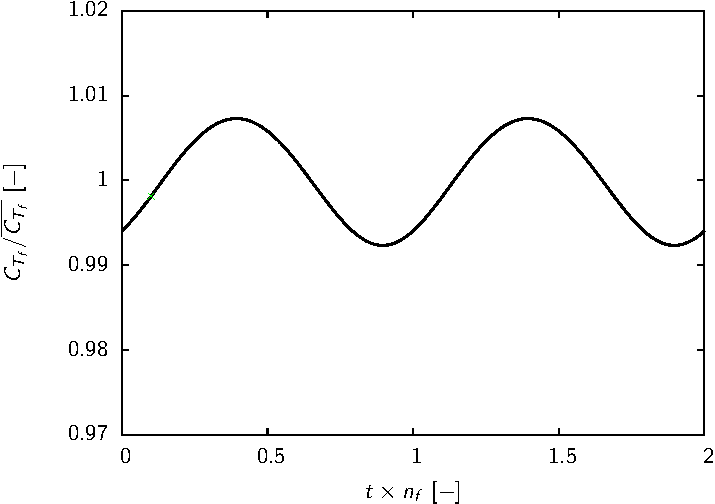
\includegraphics[width=.4\textwidth]{DREAM_HS_TSM_FORCES_INST_FRONT_PPT.pdf}}
  \subfigure[rear rotor]{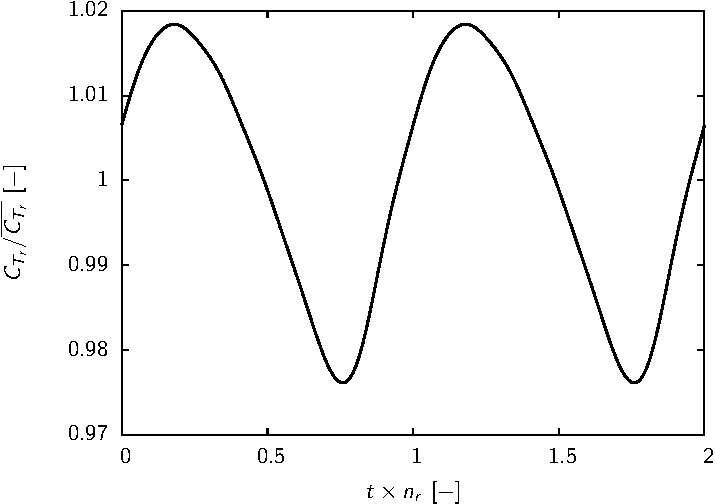
\includegraphics[width=.4\textwidth]{DREAM_HS_TSM_FORCES_INST_REAR_PPT.pdf}}
  \caption{High-speed isolated configuration: unsteadiness seen by the rotors.}
  \label{fig:dream_hs_hb_unst_coeff}
\end{figure}
The envelop of the unsteadiness is $\pm 1\%$ on the front rotor
and $\pm 2\%$ on the rear rotor. This has to be compared to 
the $\pm 3 \permil$ observed for both rotors on the low-speed configuration.
The amplitude of unsteadiness is doubled on the rear rotor,
compared to the front rotor one,
meaning that the wake effects are much stronger than the
potential ones when considering the high-speed inflow condition.
The analysis of the shape of the unsteady thrust coefficient
reveals that it is close to a sine shape function for the front
rotor.

\subsection{Two-dimensional results: harmonic blade response}
\label{sub:dream_hs_hb_blade_response}

To further analyze the unsteadinesses perceived by both rotors,
a discrete Fourier transform of the first harmonic of the static pressure
of the opposite blade passing frequency is shown in 
Figure~\ref{fig:dream_hs_hb_blade_response}. Note that the
scale is different for the front and the rear rotors.
\begin{figure}[htp]
 \ra{1.3} \centering
 \begin{tabular}{cccc}
    \multicolumn{2}{c}{\includegraphics[width=0.3\textwidth]{dream_HS_blade_resp_scale_H01_front.pdf}} &
    \multicolumn{2}{c}{\includegraphics[width=0.3\textwidth]{dream_HS_blade_resp_scale_H01_rear.pdf}} \\
    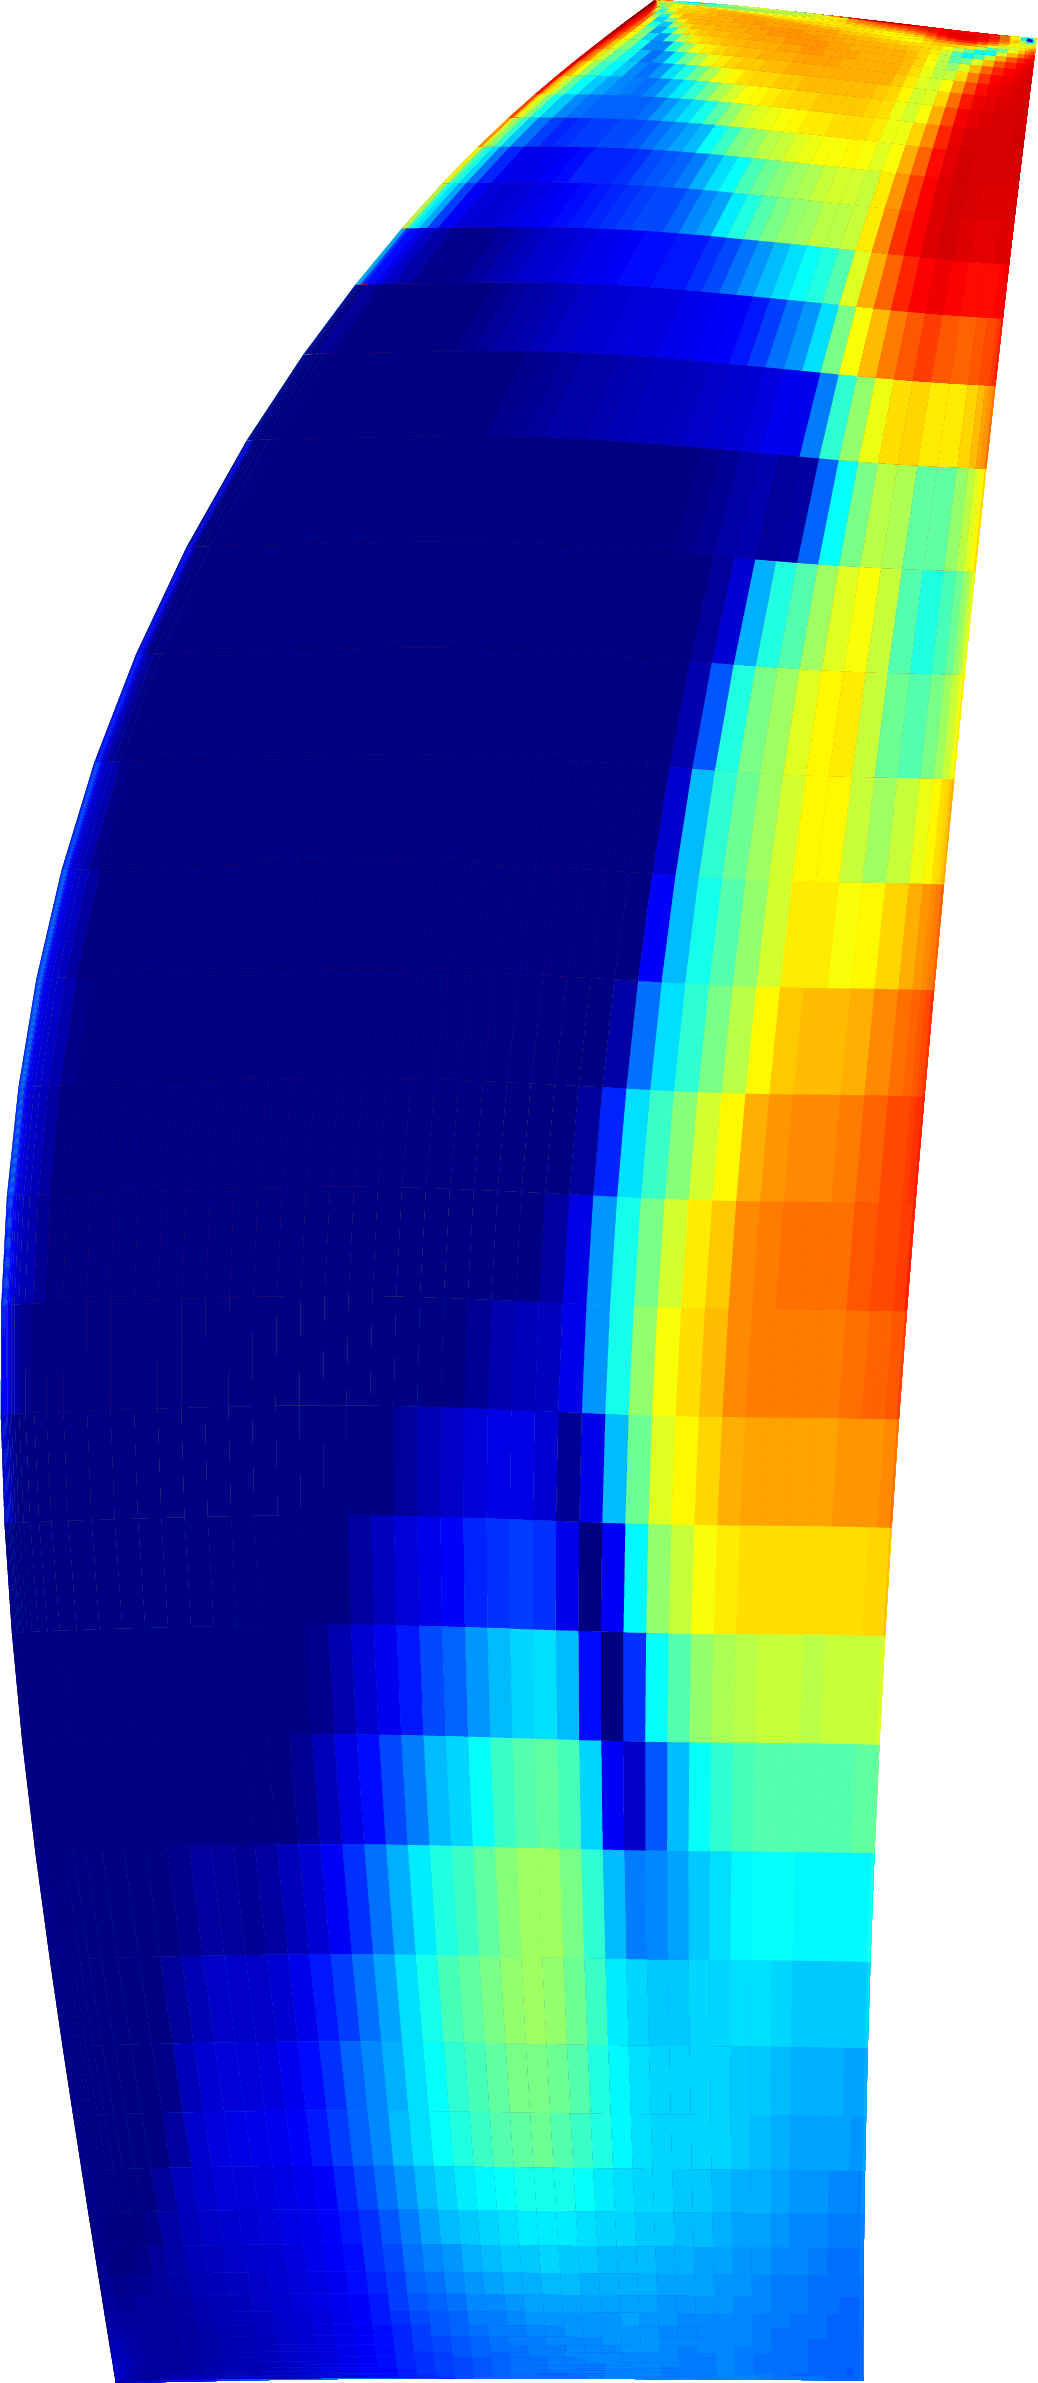
\includegraphics[width=0.15\textwidth]{DREAM_HS_TSM_N7_roe2_sa_blade_response_front_H01_SS.png}
    & 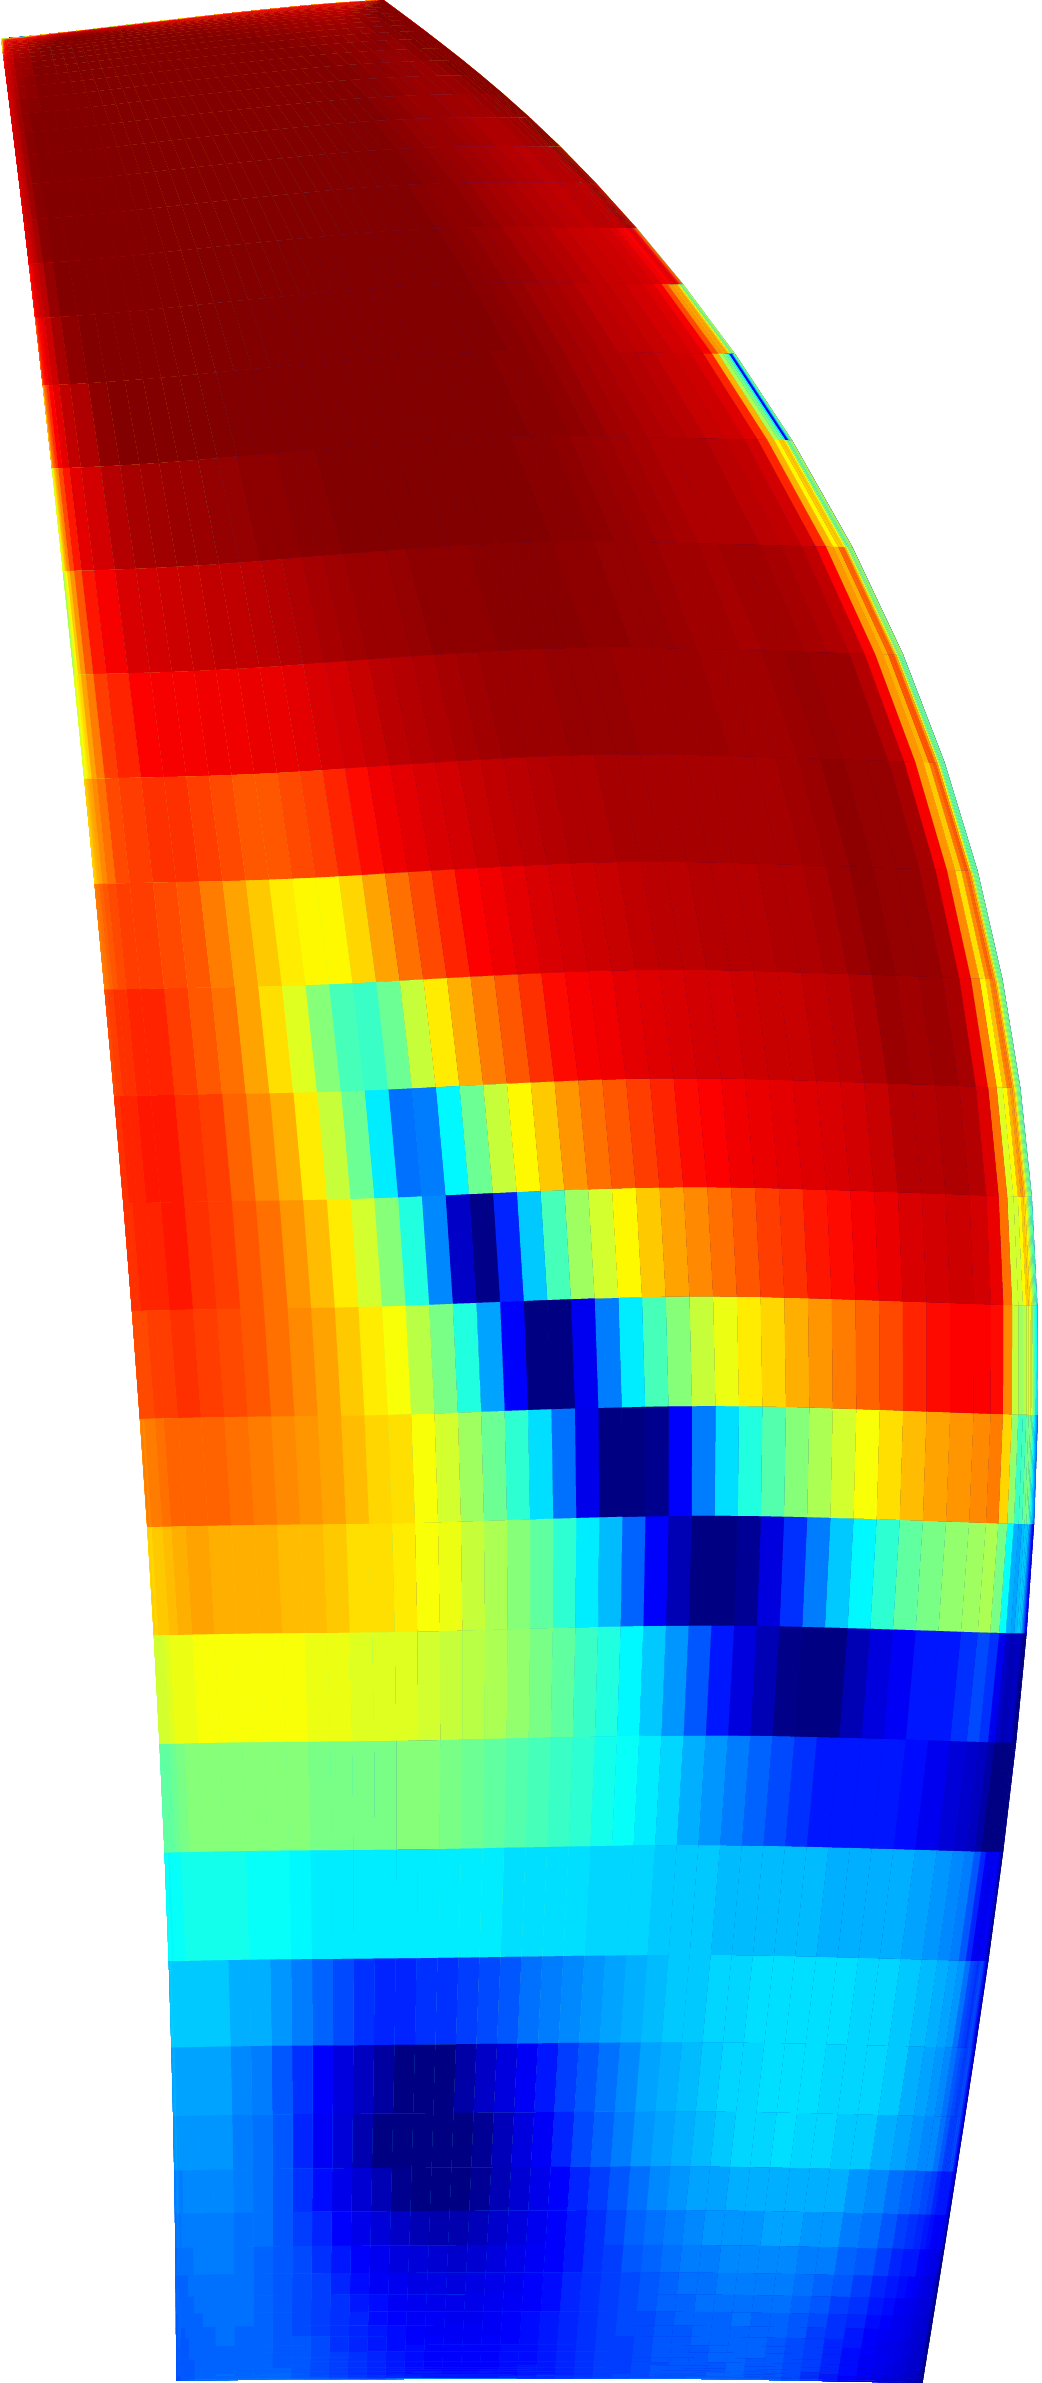
\includegraphics[width=0.15\textwidth]{DREAM_HS_TSM_N7_roe2_sa_blade_response_front_H01_PS.png}
    & 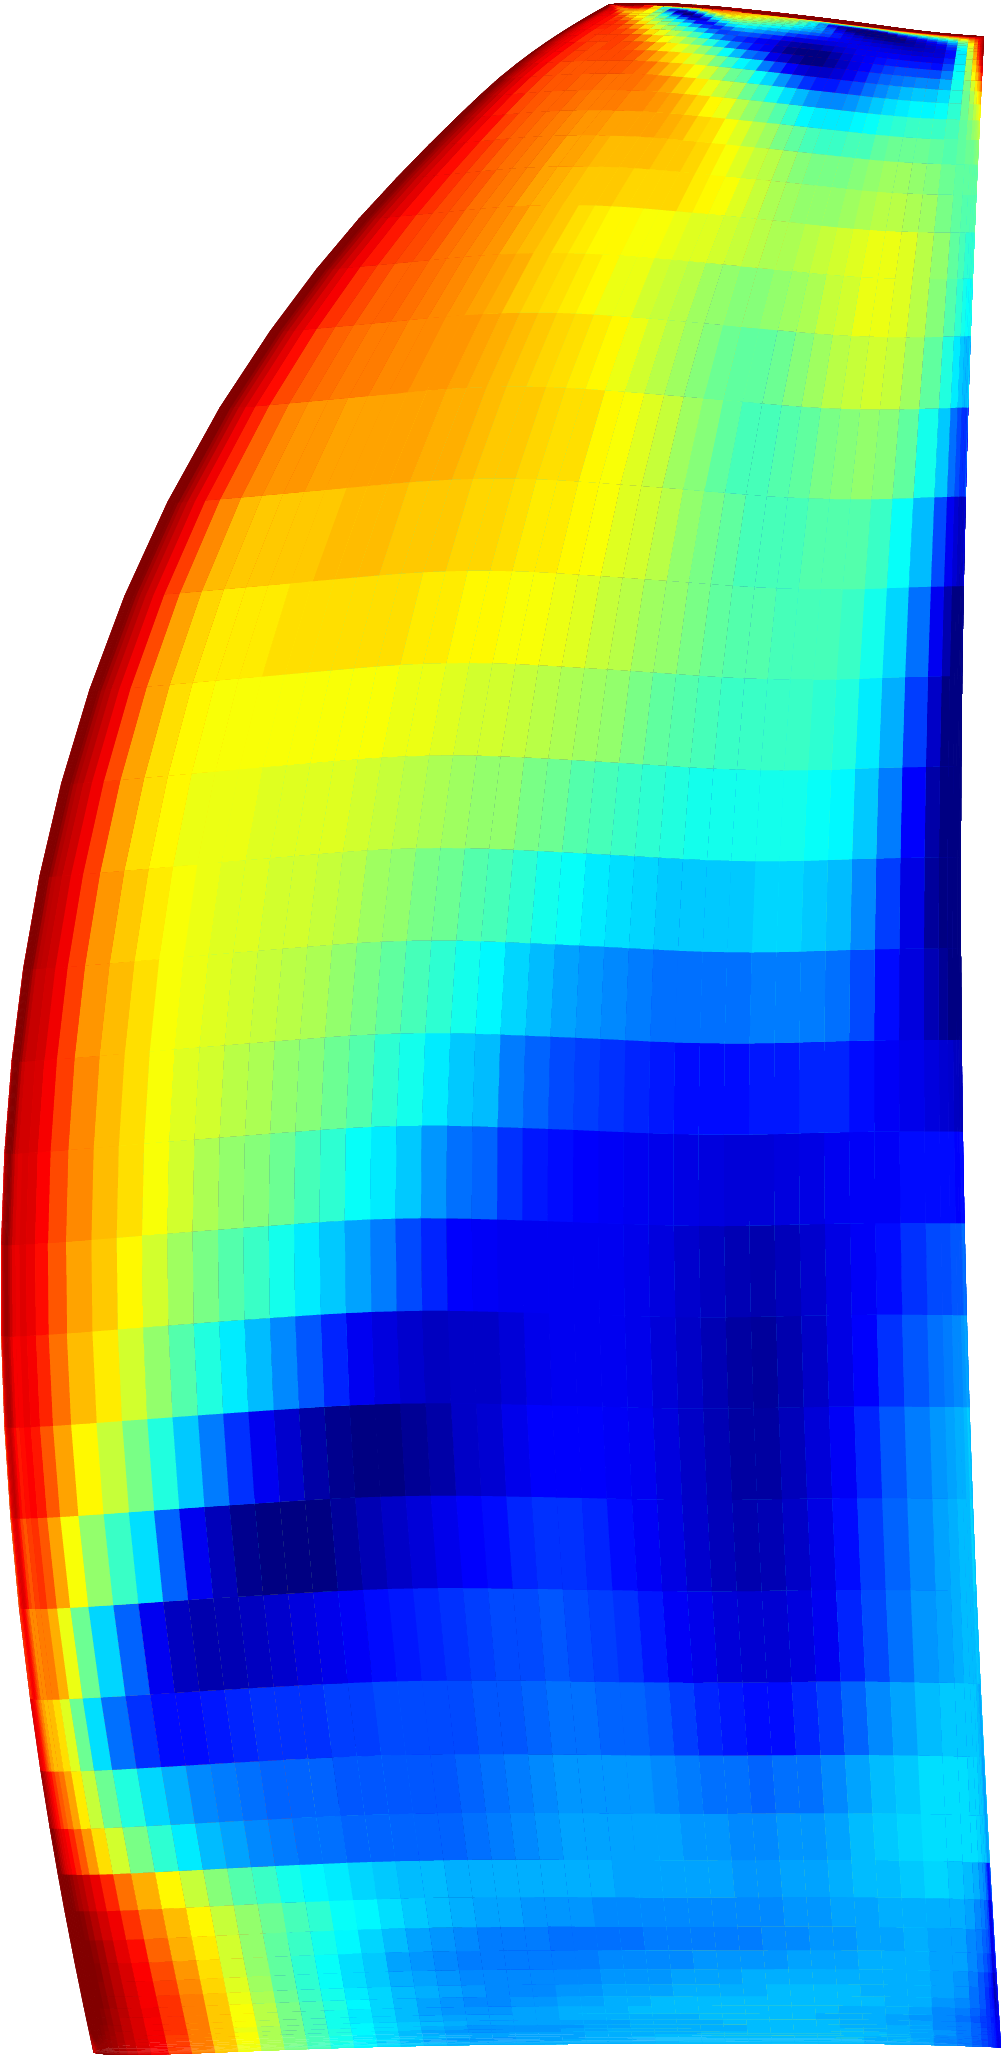
\includegraphics[width=0.15\textwidth]{DREAM_HS_TSM_N7_roe2_sa_blade_response_rear_H01_PS.png}
    & 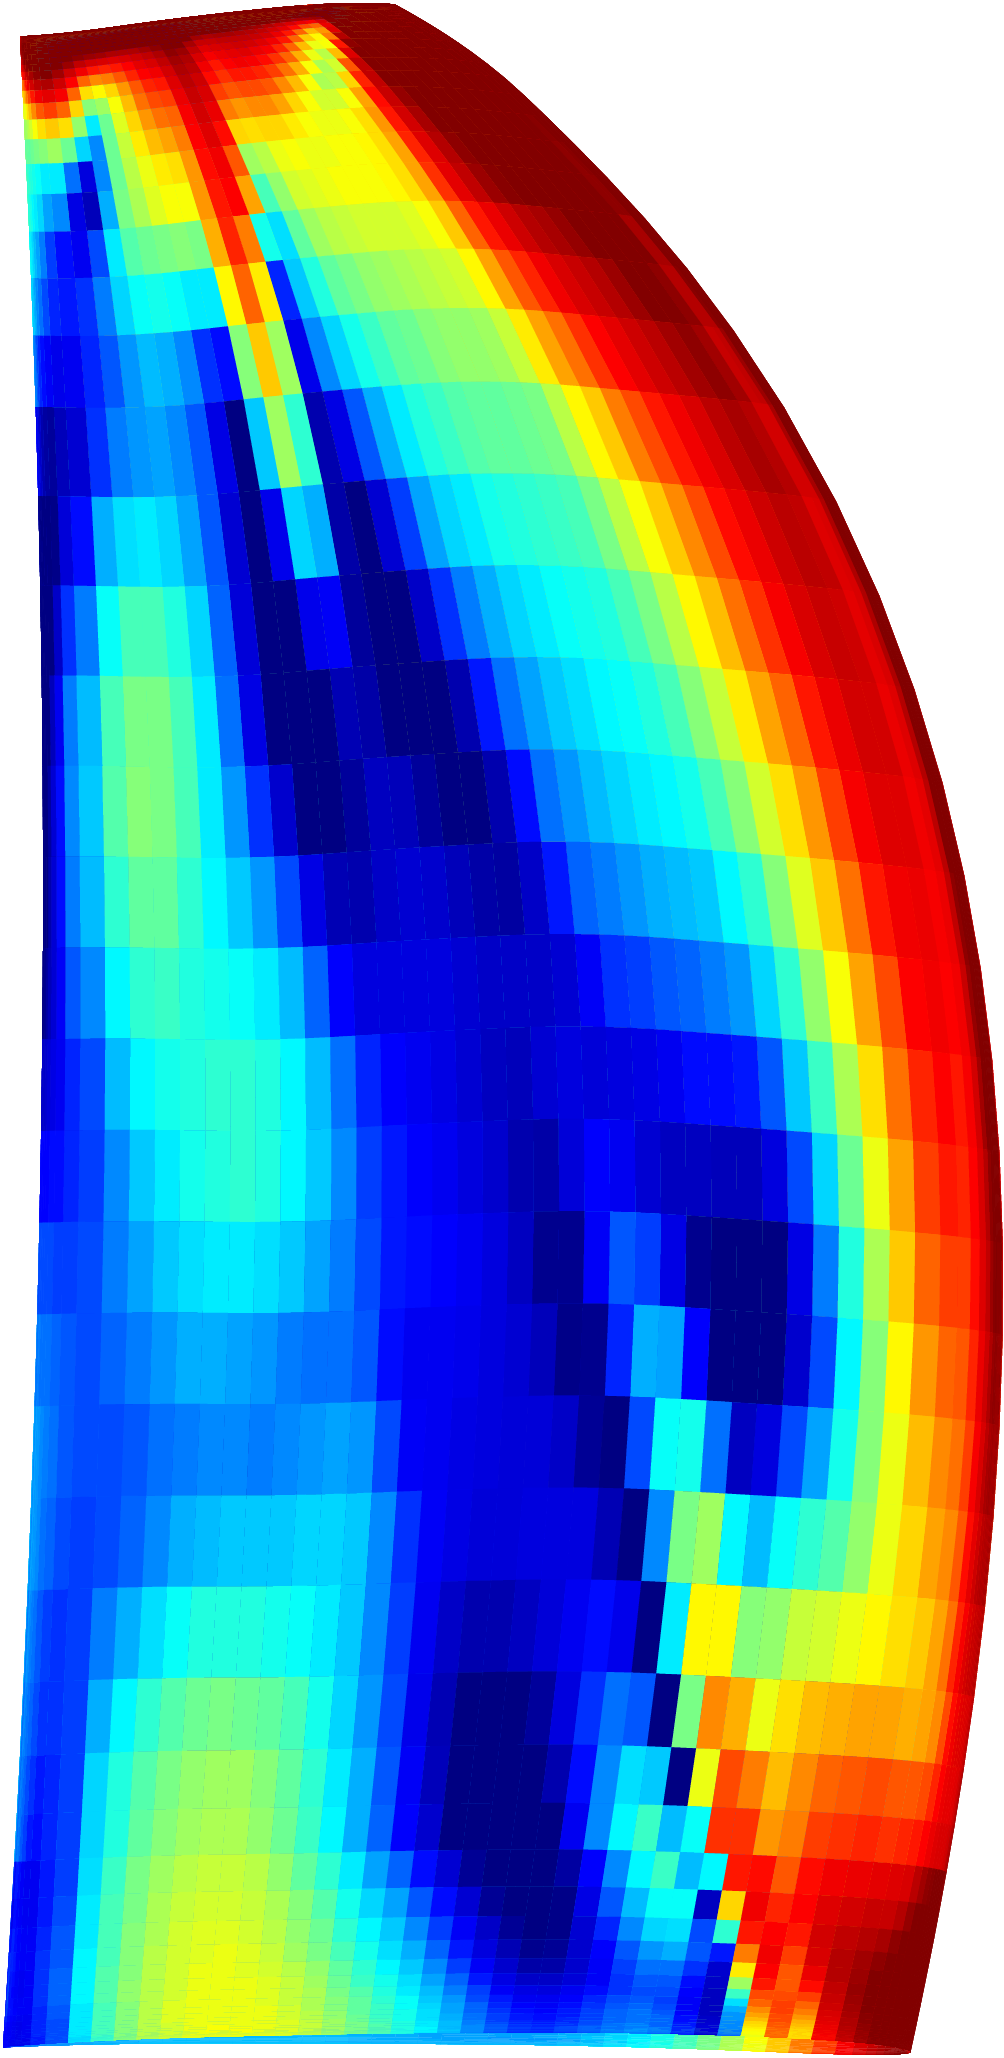
\includegraphics[width=0.15\textwidth]{DREAM_HS_TSM_N7_roe2_sa_blade_response_rear_H01_SS.png} \\
    \multicolumn{2}{c}{\emph{Front rotor blade}}
    & \multicolumn{2}{c}{\emph{Rear rotor blade}} \\
    suction side & pressure side & pressure side & suction side
 \end{tabular}
 \caption{High-speed isolated configuration: harmonic response of the front
 rotor blades.}
 \label{fig:dream_hs_hb_blade_response}
\end{figure}

On the front rotor, the maximum amplitude
is observed at the tip of the pressure side. This is consistent
with the observation made on the low-speed configuration, where
the pressure side was more exposed to pressure variations.
In fact, the suction side is shielded 
from the downstream disturbances by the blade angle of attack.
The suction side is not only shielded by the blade angle
of attack but also by the shock that forms around 
$x/c \approx 0.7$ for relative span greater than $40\%$,
as mentioned in Sec.~\ref{sub:dream_hs_blades}. For
relative span smaller than $40\%$, the shock is closer the
leading edge, hence the pressure unsteadiness going
upstream. On the tip of the front rotor blade,
a vortex is formed that leaves the blades from the pressure
side to the suction side. It helps increasing
the pressure on the suction side, alleviating the formation
of a shock. Therefore, at the tip of the blade, the pressure variations
are observed all the way to the leading edge.

On the rear rotor, the suction side of the blade 
shows a large structure of high unsteadiness near 
the leading edge. This is attributed to the wake passing.
In opposite, a large low amplitude region is observed in the
middle of the suction side of the blade. This is attributed
to the shielding effect of the shock. In fact, the shock is 
a discontinuity that prevents unsteady effects to affect the
blade. On the pressure side, the level of unsteadiness is much larger
than the one observed on the low-speed configuration, relatively
to the suction side level. Actually, the smaller
angle of attack of the blades might explain this high level.
Similar as the suction side of the front rotor
blade that are shielded from potential effects coming
from the rear rotor blades, the pressure side is relatively
less affected by the wake passing than the suction side is.
However, for the high-speed configuration, the angle of
attack is smaller as said in Sec.~\ref{sec:dream_hs_presentation}.
Therefore, the unsteady effects hitting the suction side of the
rear rotor blades are more prone to affect the pressure side
too. Moreover, as no shock is present on the pressure side,
these unsteadinesses affects the whole chord. 

\subsection{Two-dimensional results: axial cuts}
\label{sub:dream_hs_hb_axial_cuts}

Axial cuts of entropy are shown in 
Figure~\ref{fig:dream_hs_hb_axial_cut_entropy} for several
axis positions and compared to steady computation results.
\begin{figure}[htp]
 \ra{1.3} \centering
 \begin{tabular}{rcc}
   & steady
   & HB $N=4$ \\
   \rotatebox{90}{\qquad\qquad\qquad $P3$} & 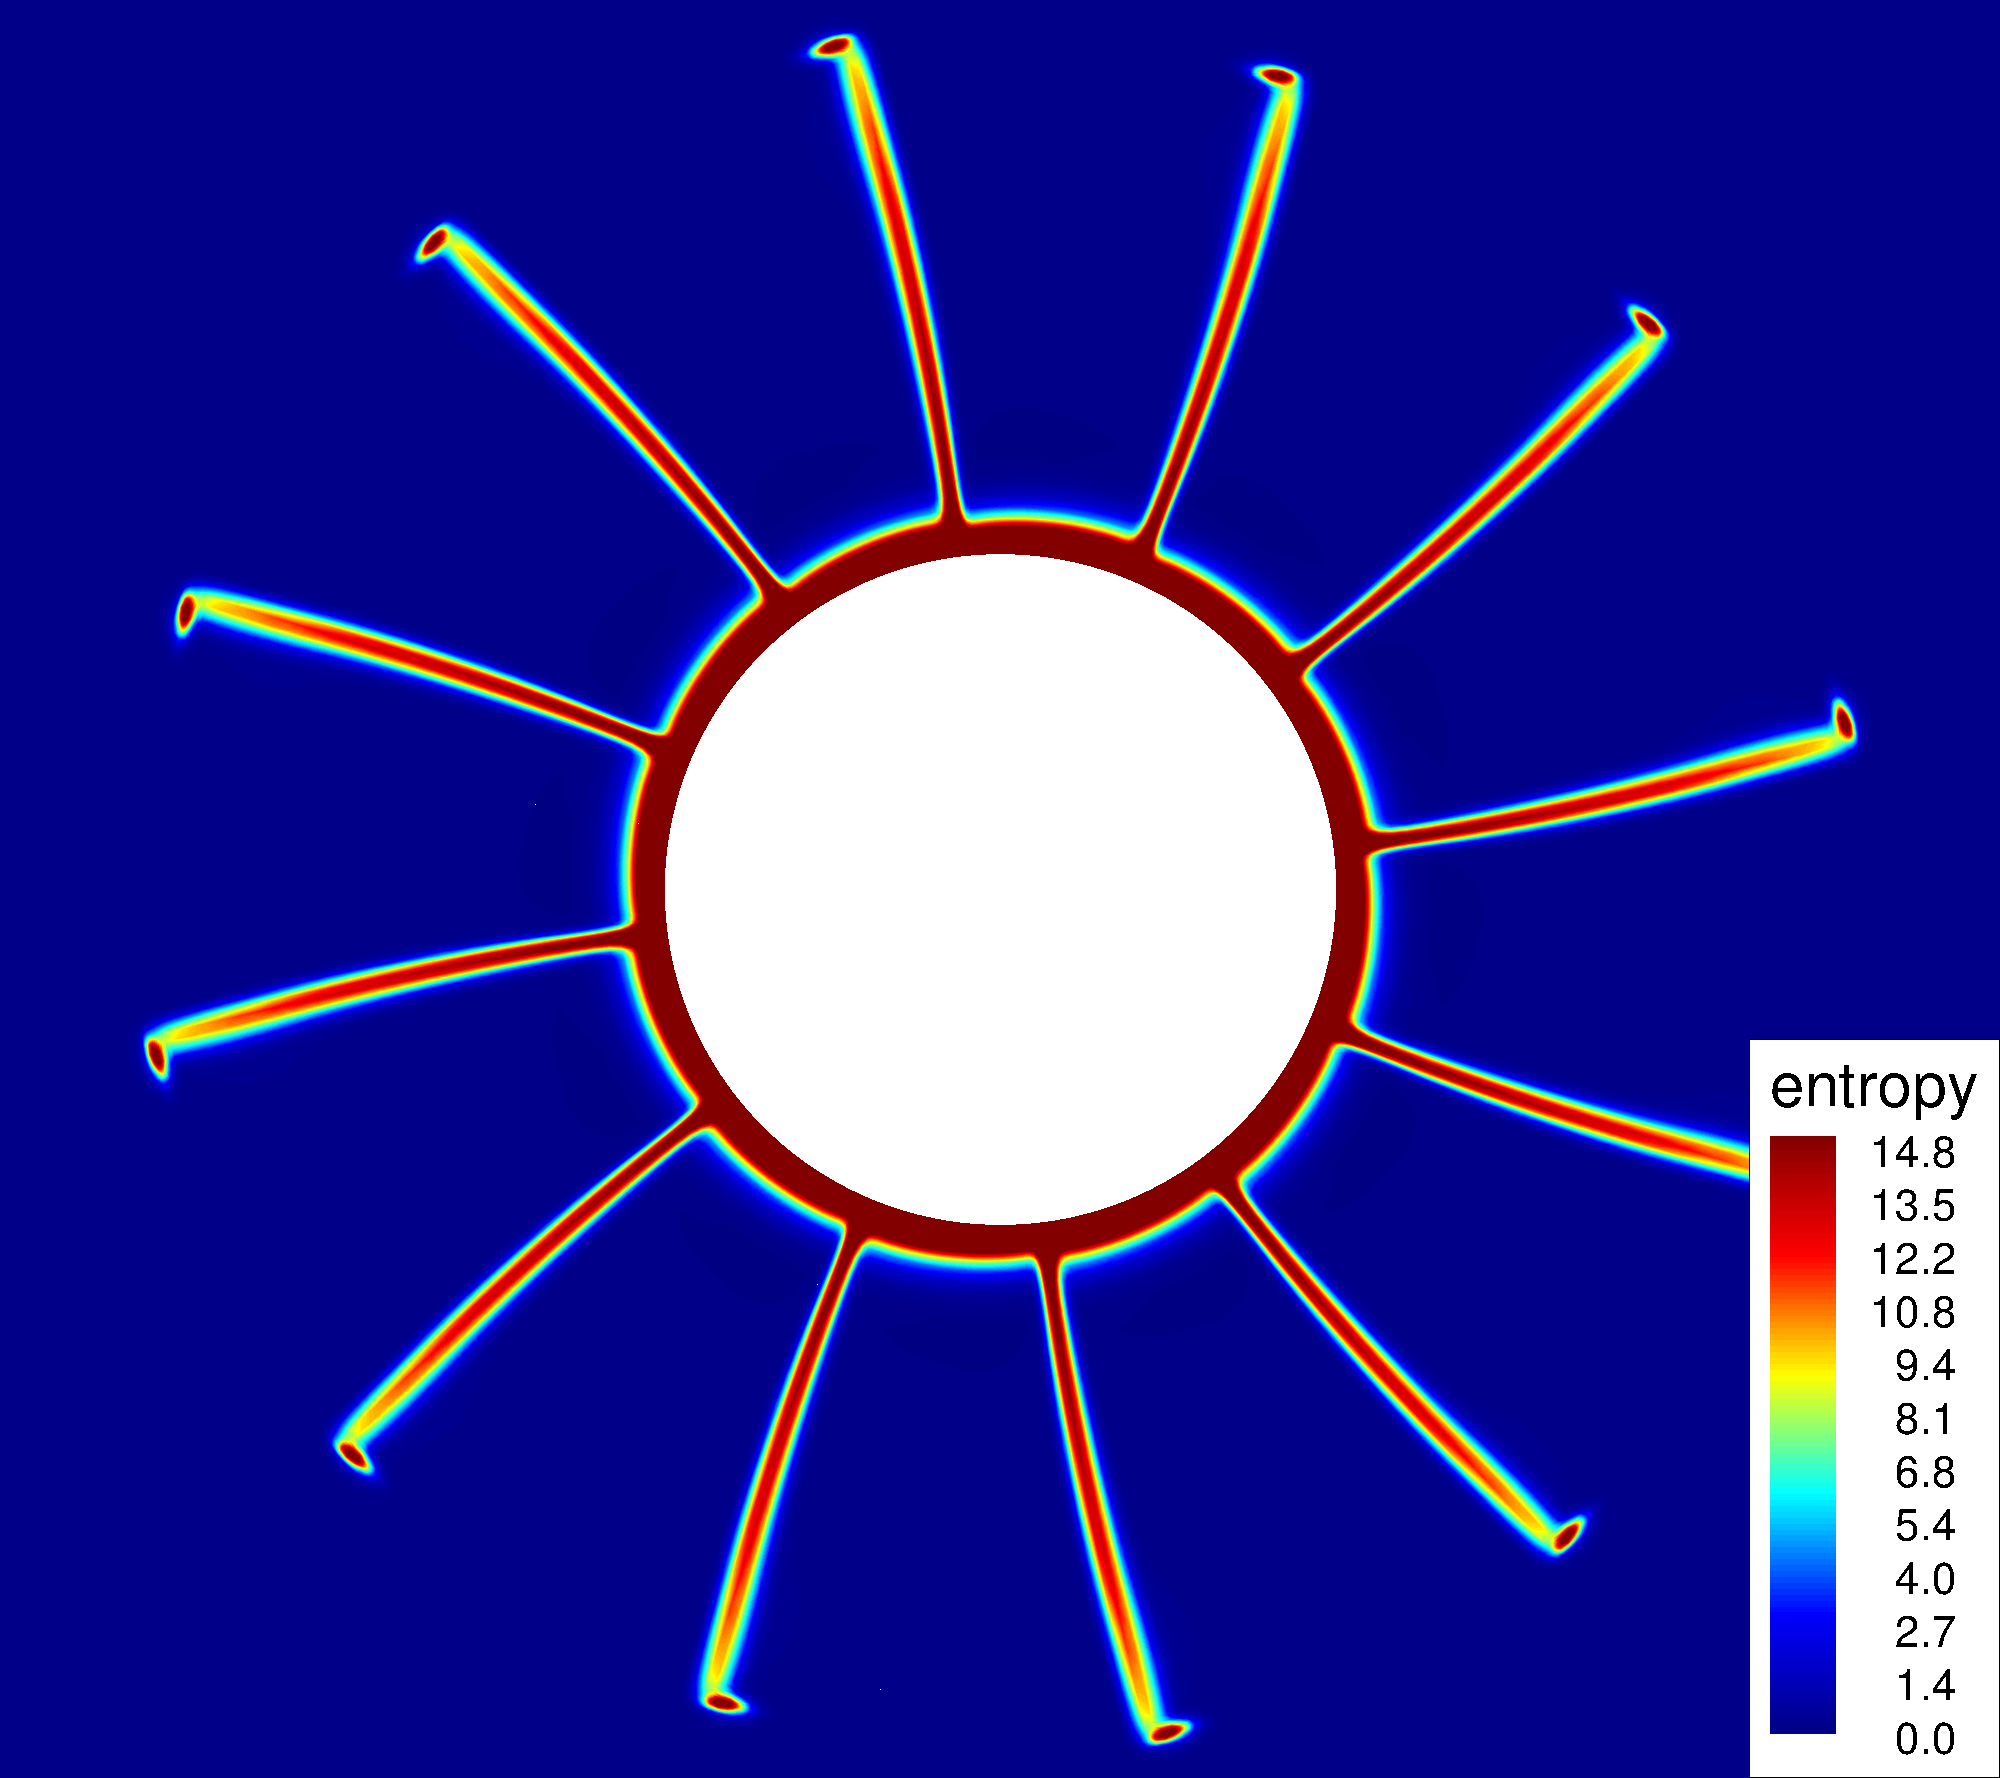
\includegraphics[width=.35\textwidth]{DREAM_HS_RANS_roe2_sa_slice_x_front_1_entropy.png}
   & 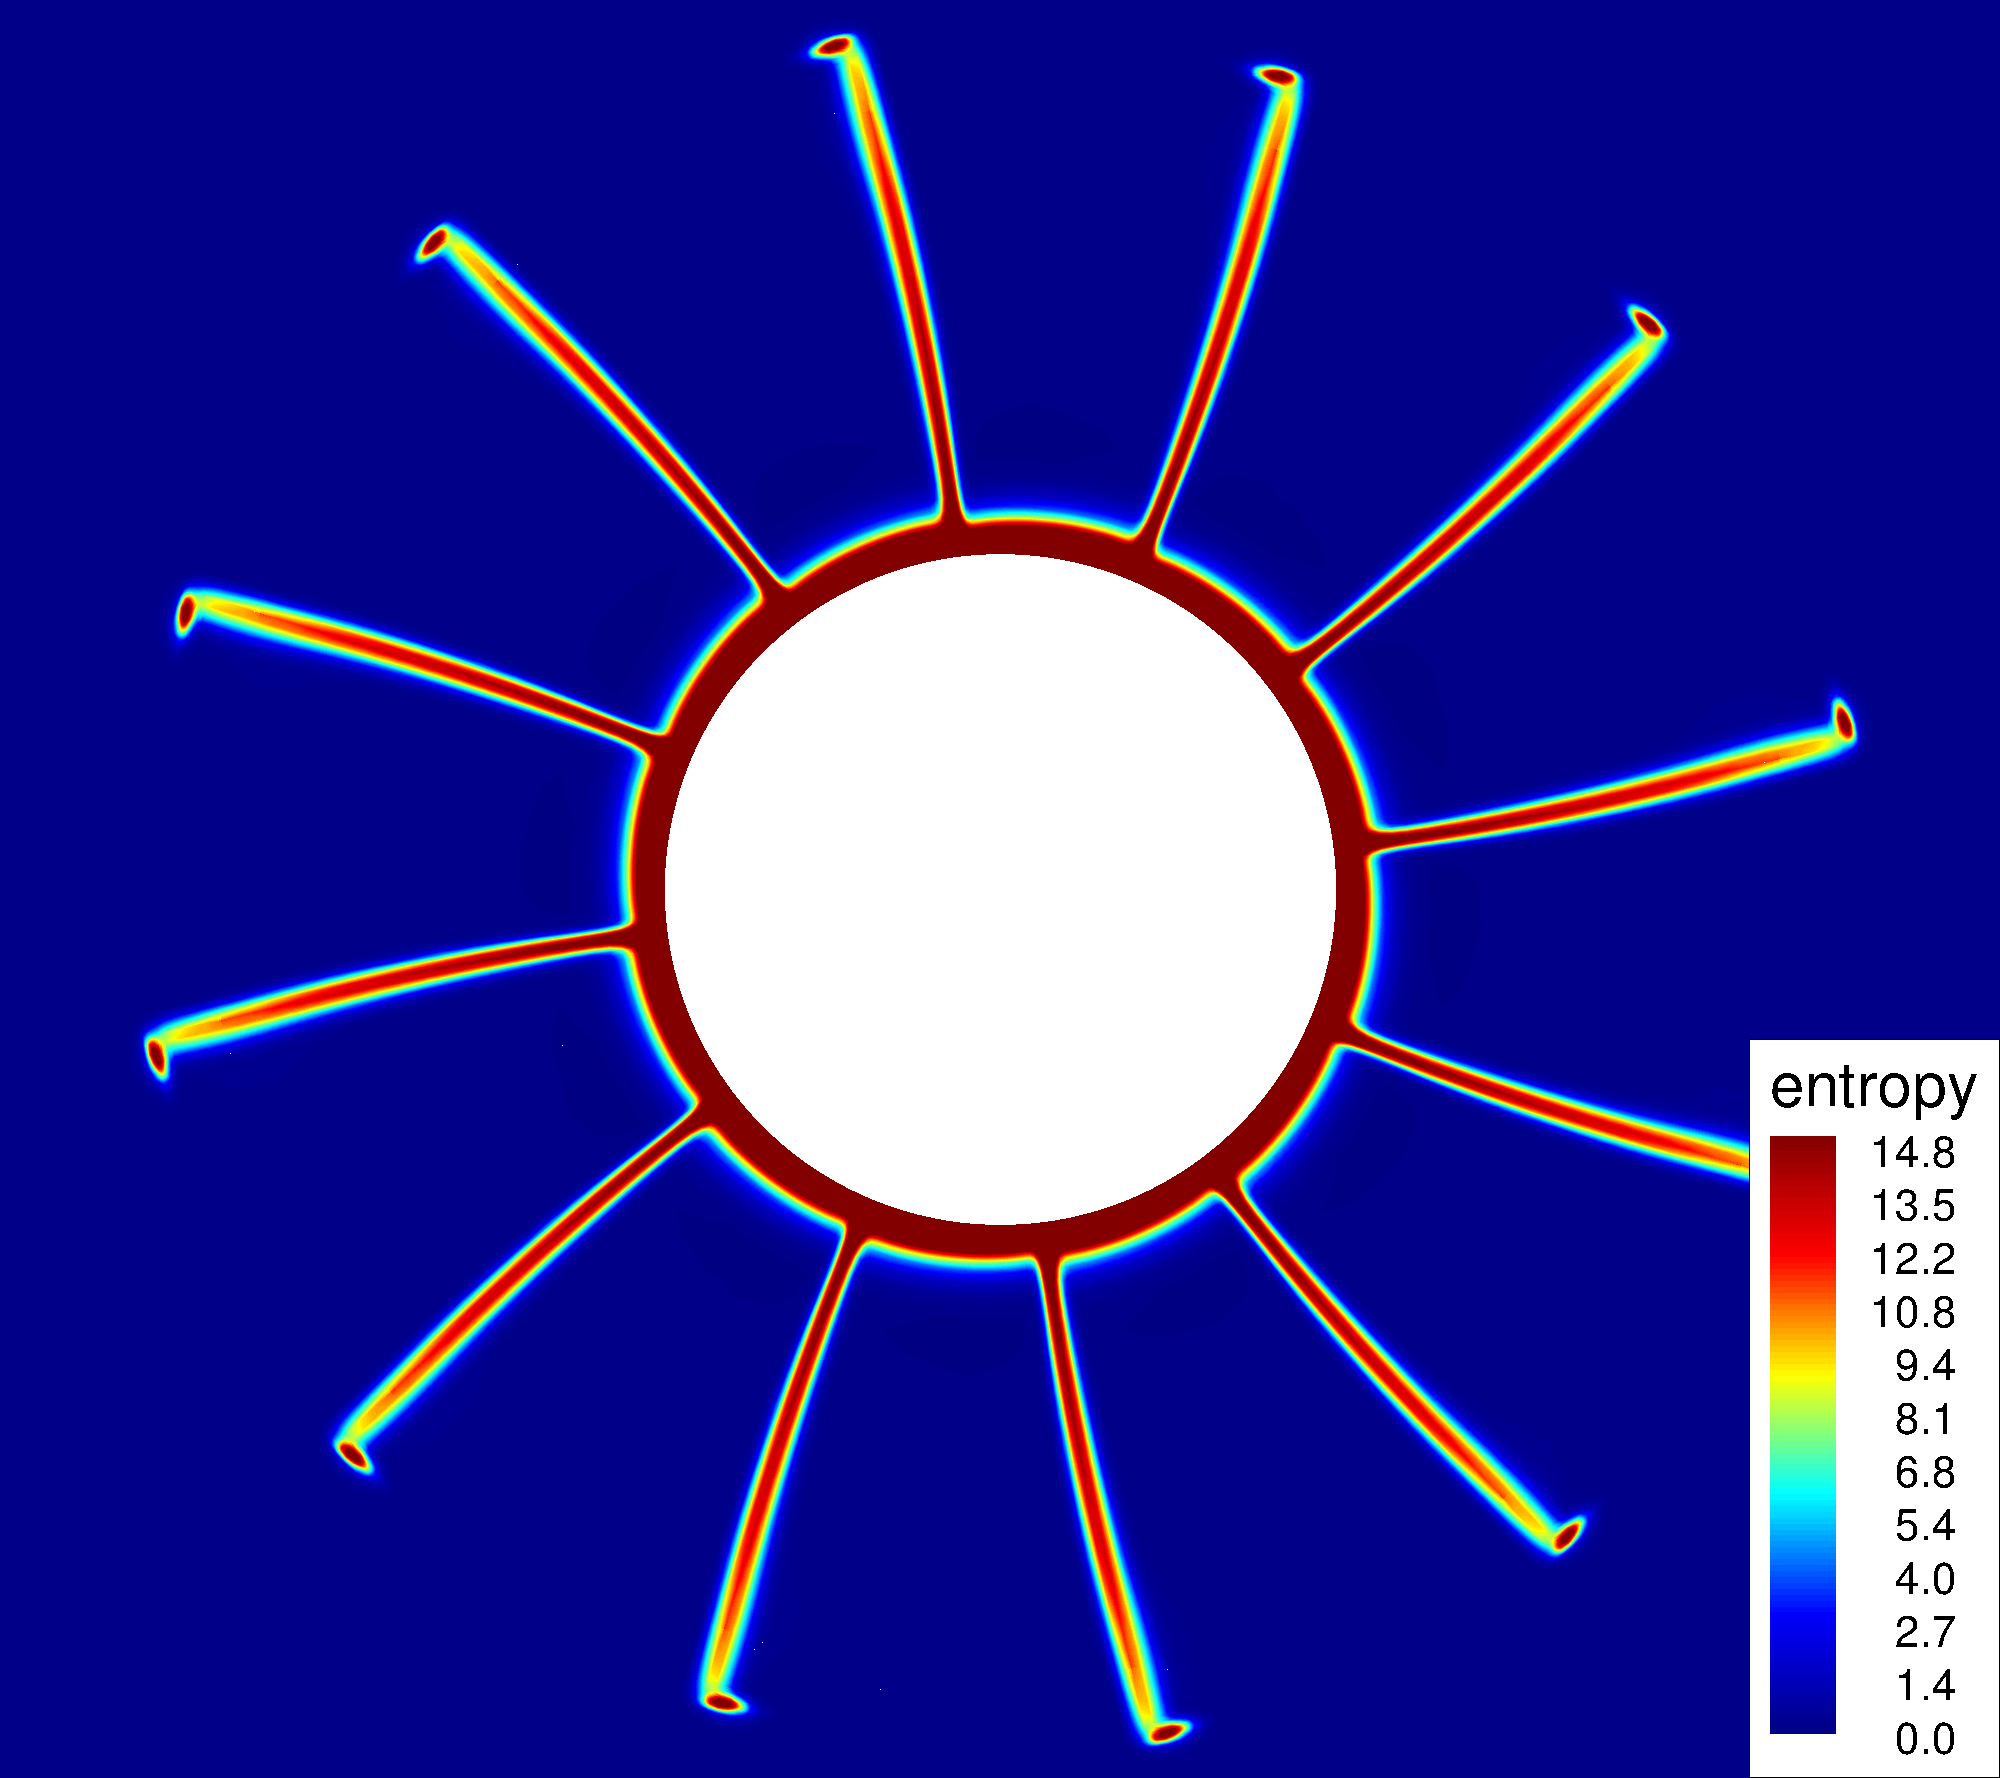
\includegraphics[width=.35\textwidth]{DREAM_HS_TSM_N7_roe2_sa_slice_x_front_1_entropy.png} \\
   \rotatebox{90}{\qquad\qquad\qquad $P4$} & 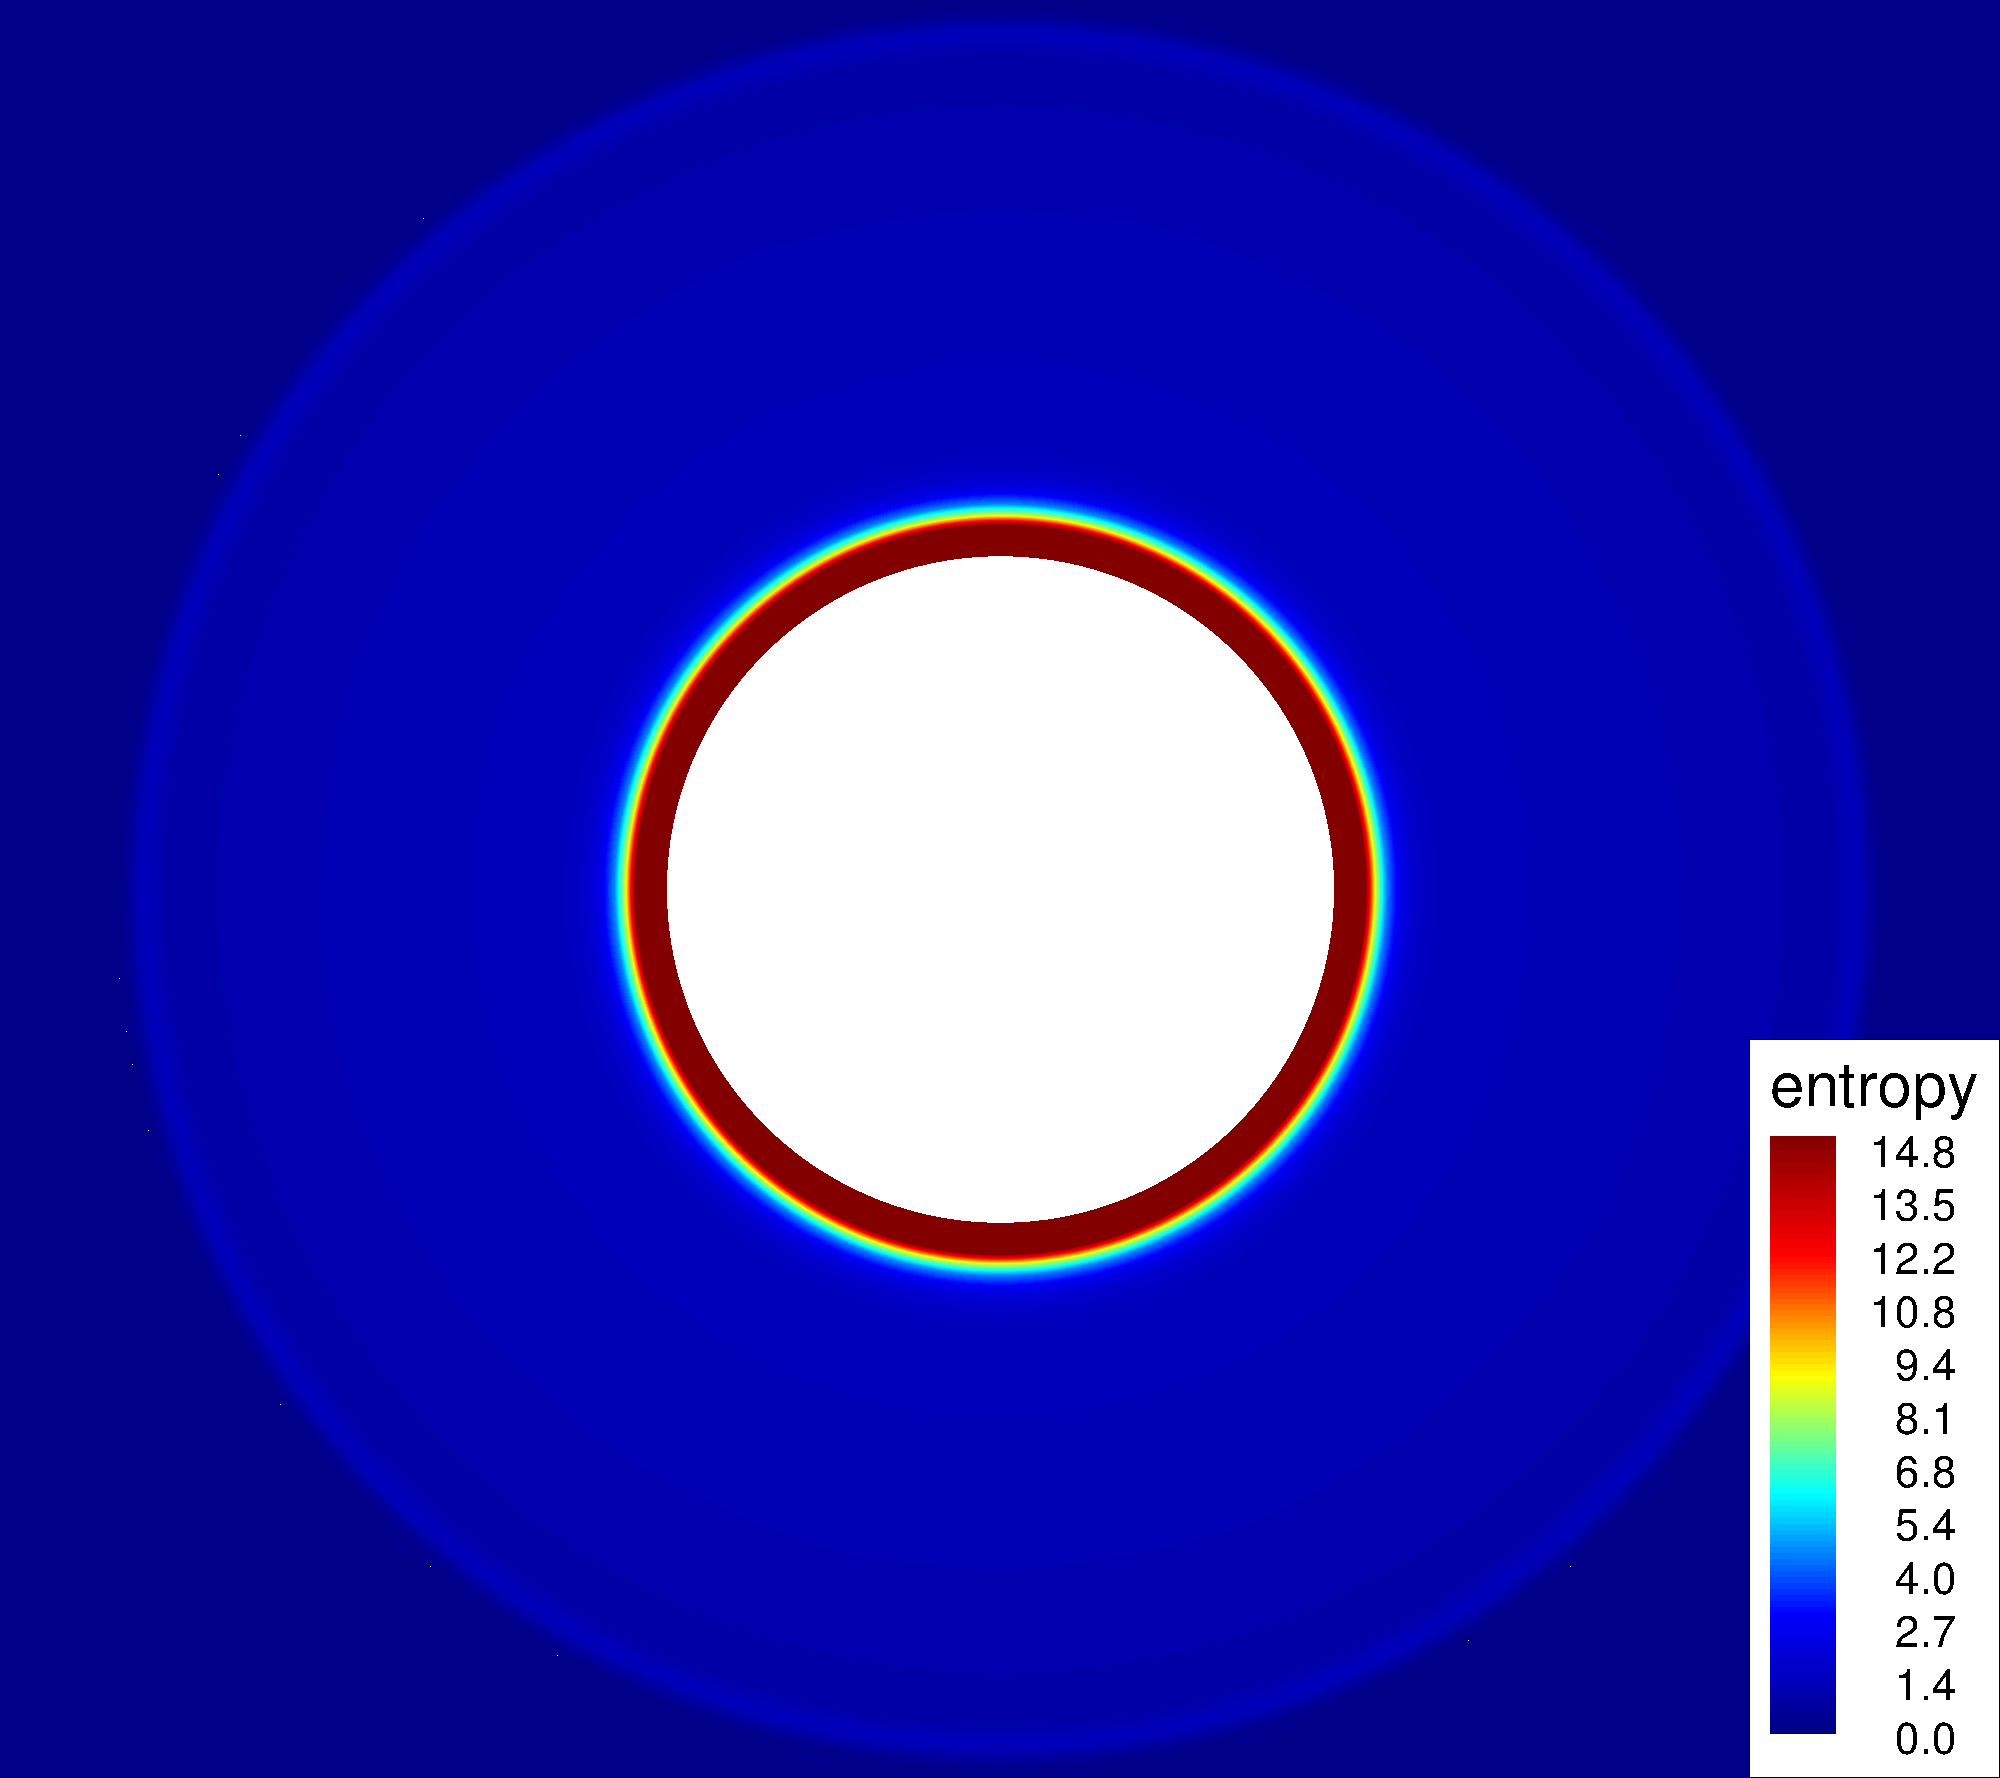
\includegraphics[width=.35\textwidth]{DREAM_HS_RANS_roe2_sa_slice_x_rear_0_entropy.png}
   & 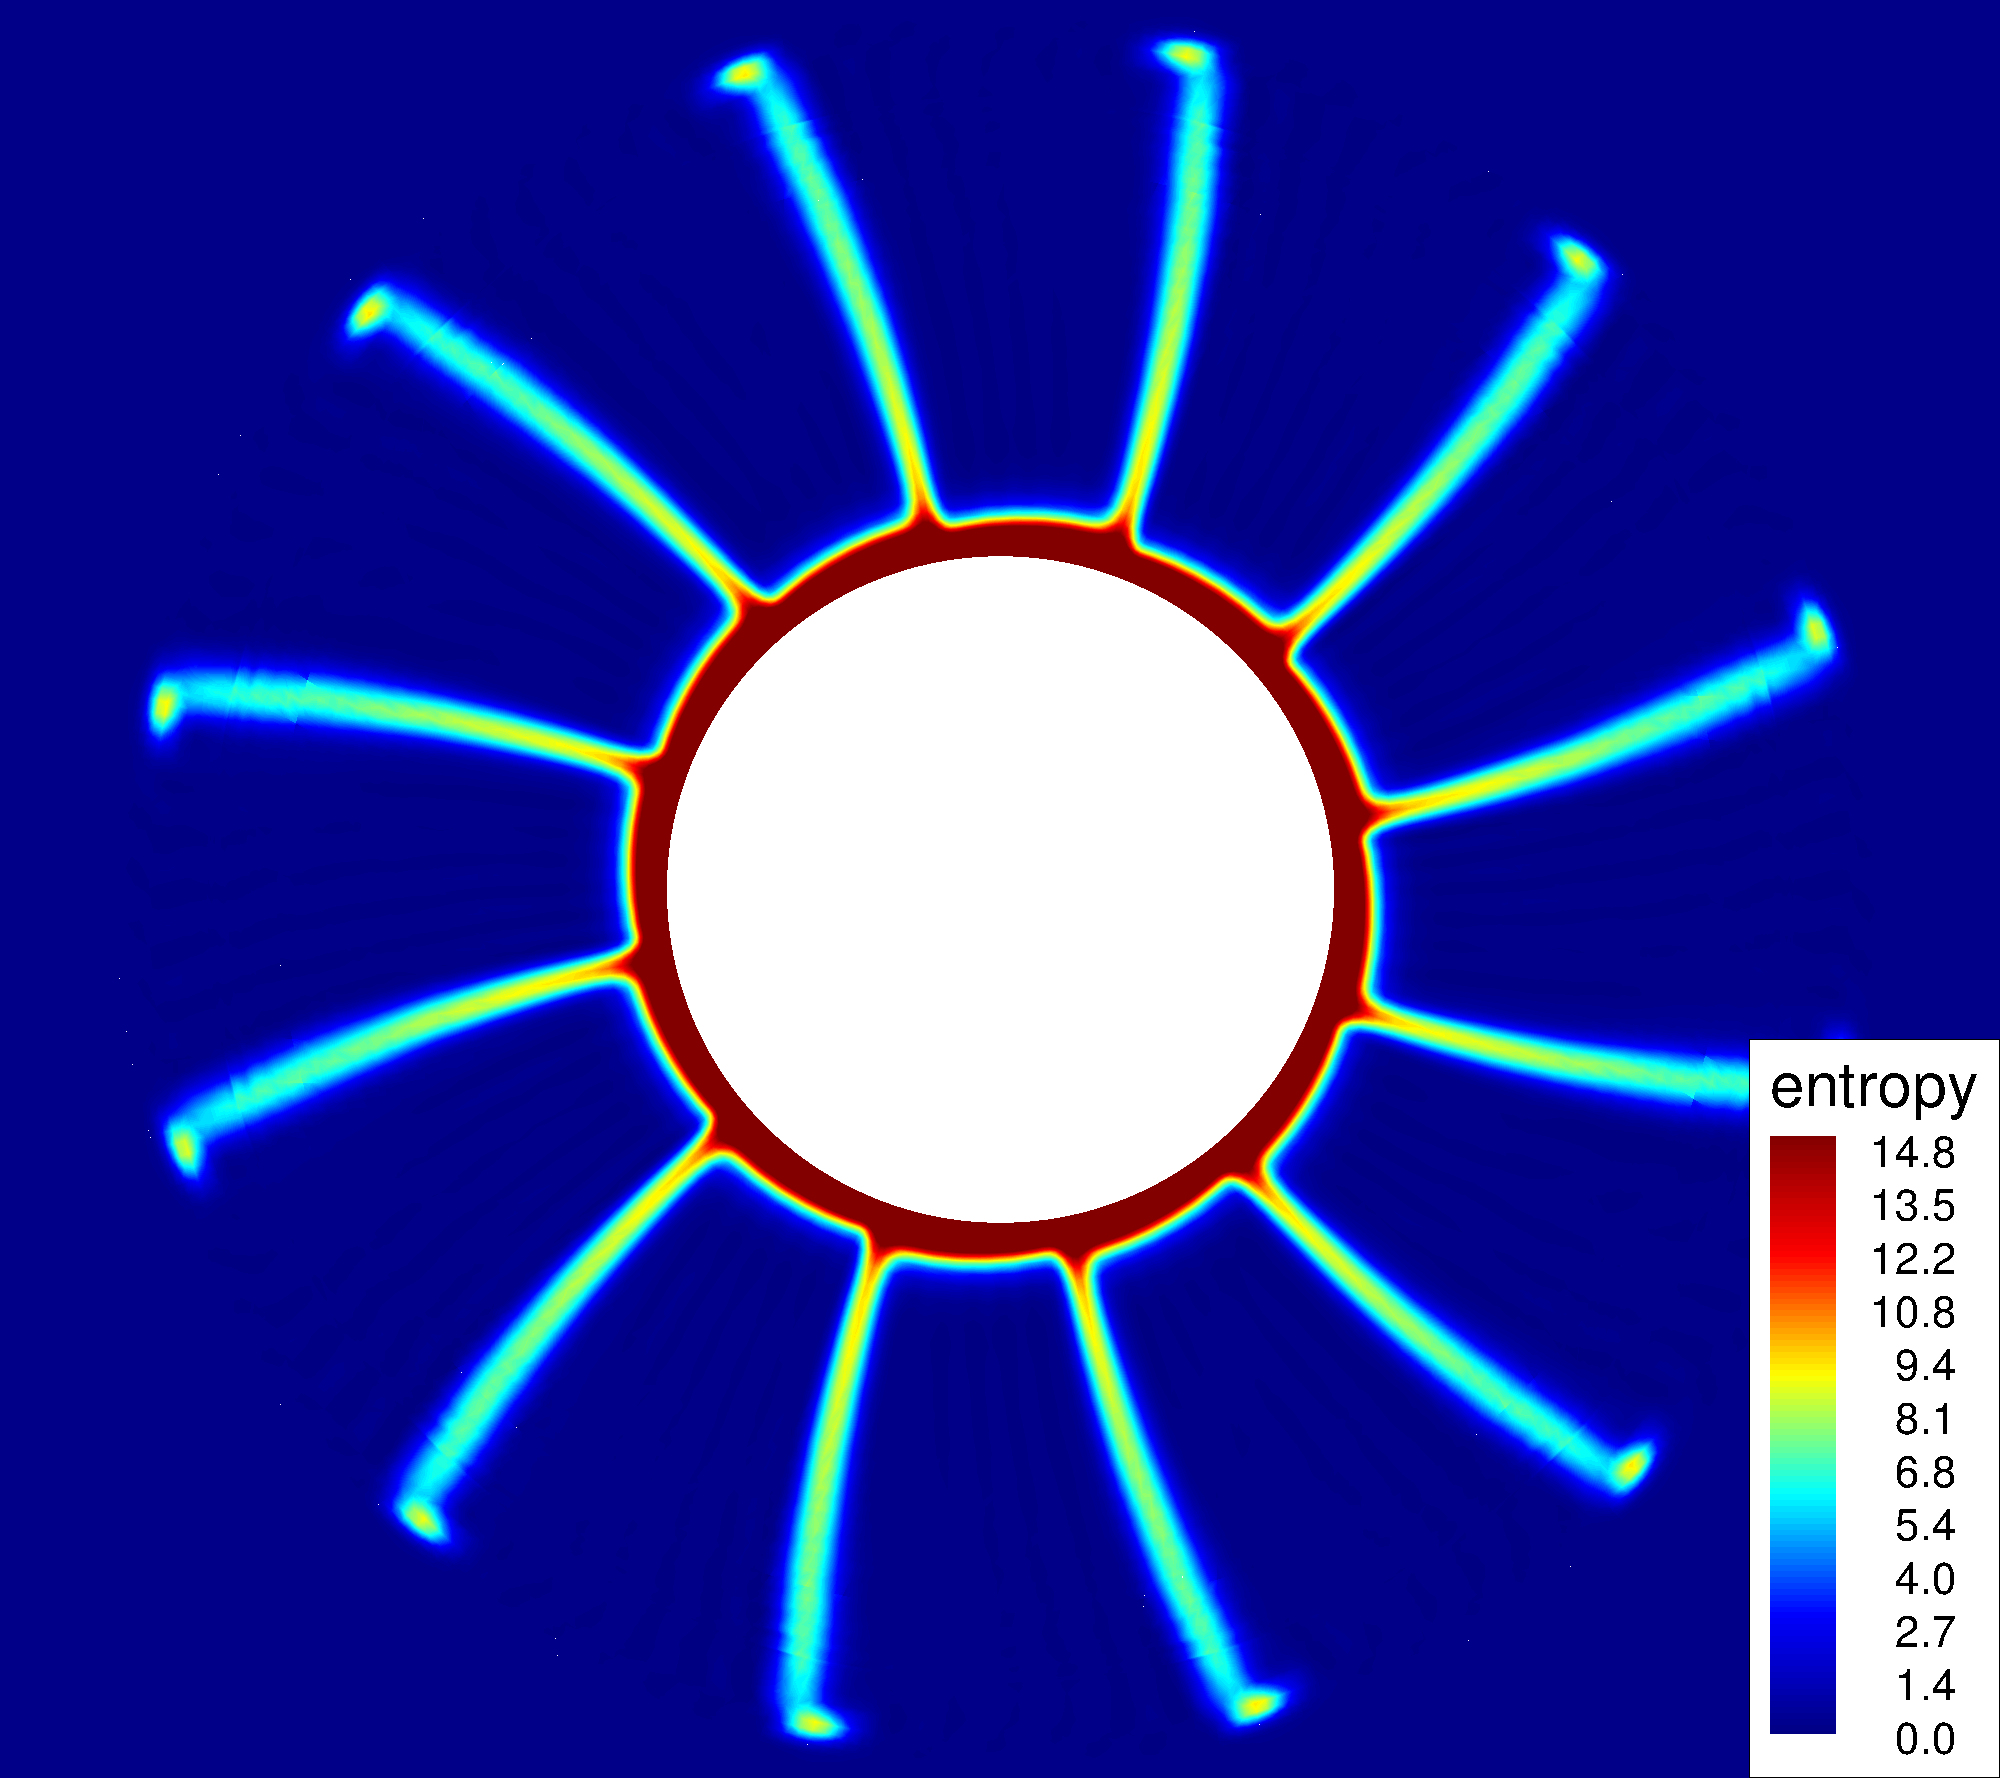
\includegraphics[width=.35\textwidth]{DREAM_HS_TSM_N7_roe2_sa_slice_x_rear_0_entropy.png} \\
   \rotatebox{90}{\qquad\qquad\qquad $P5$} & 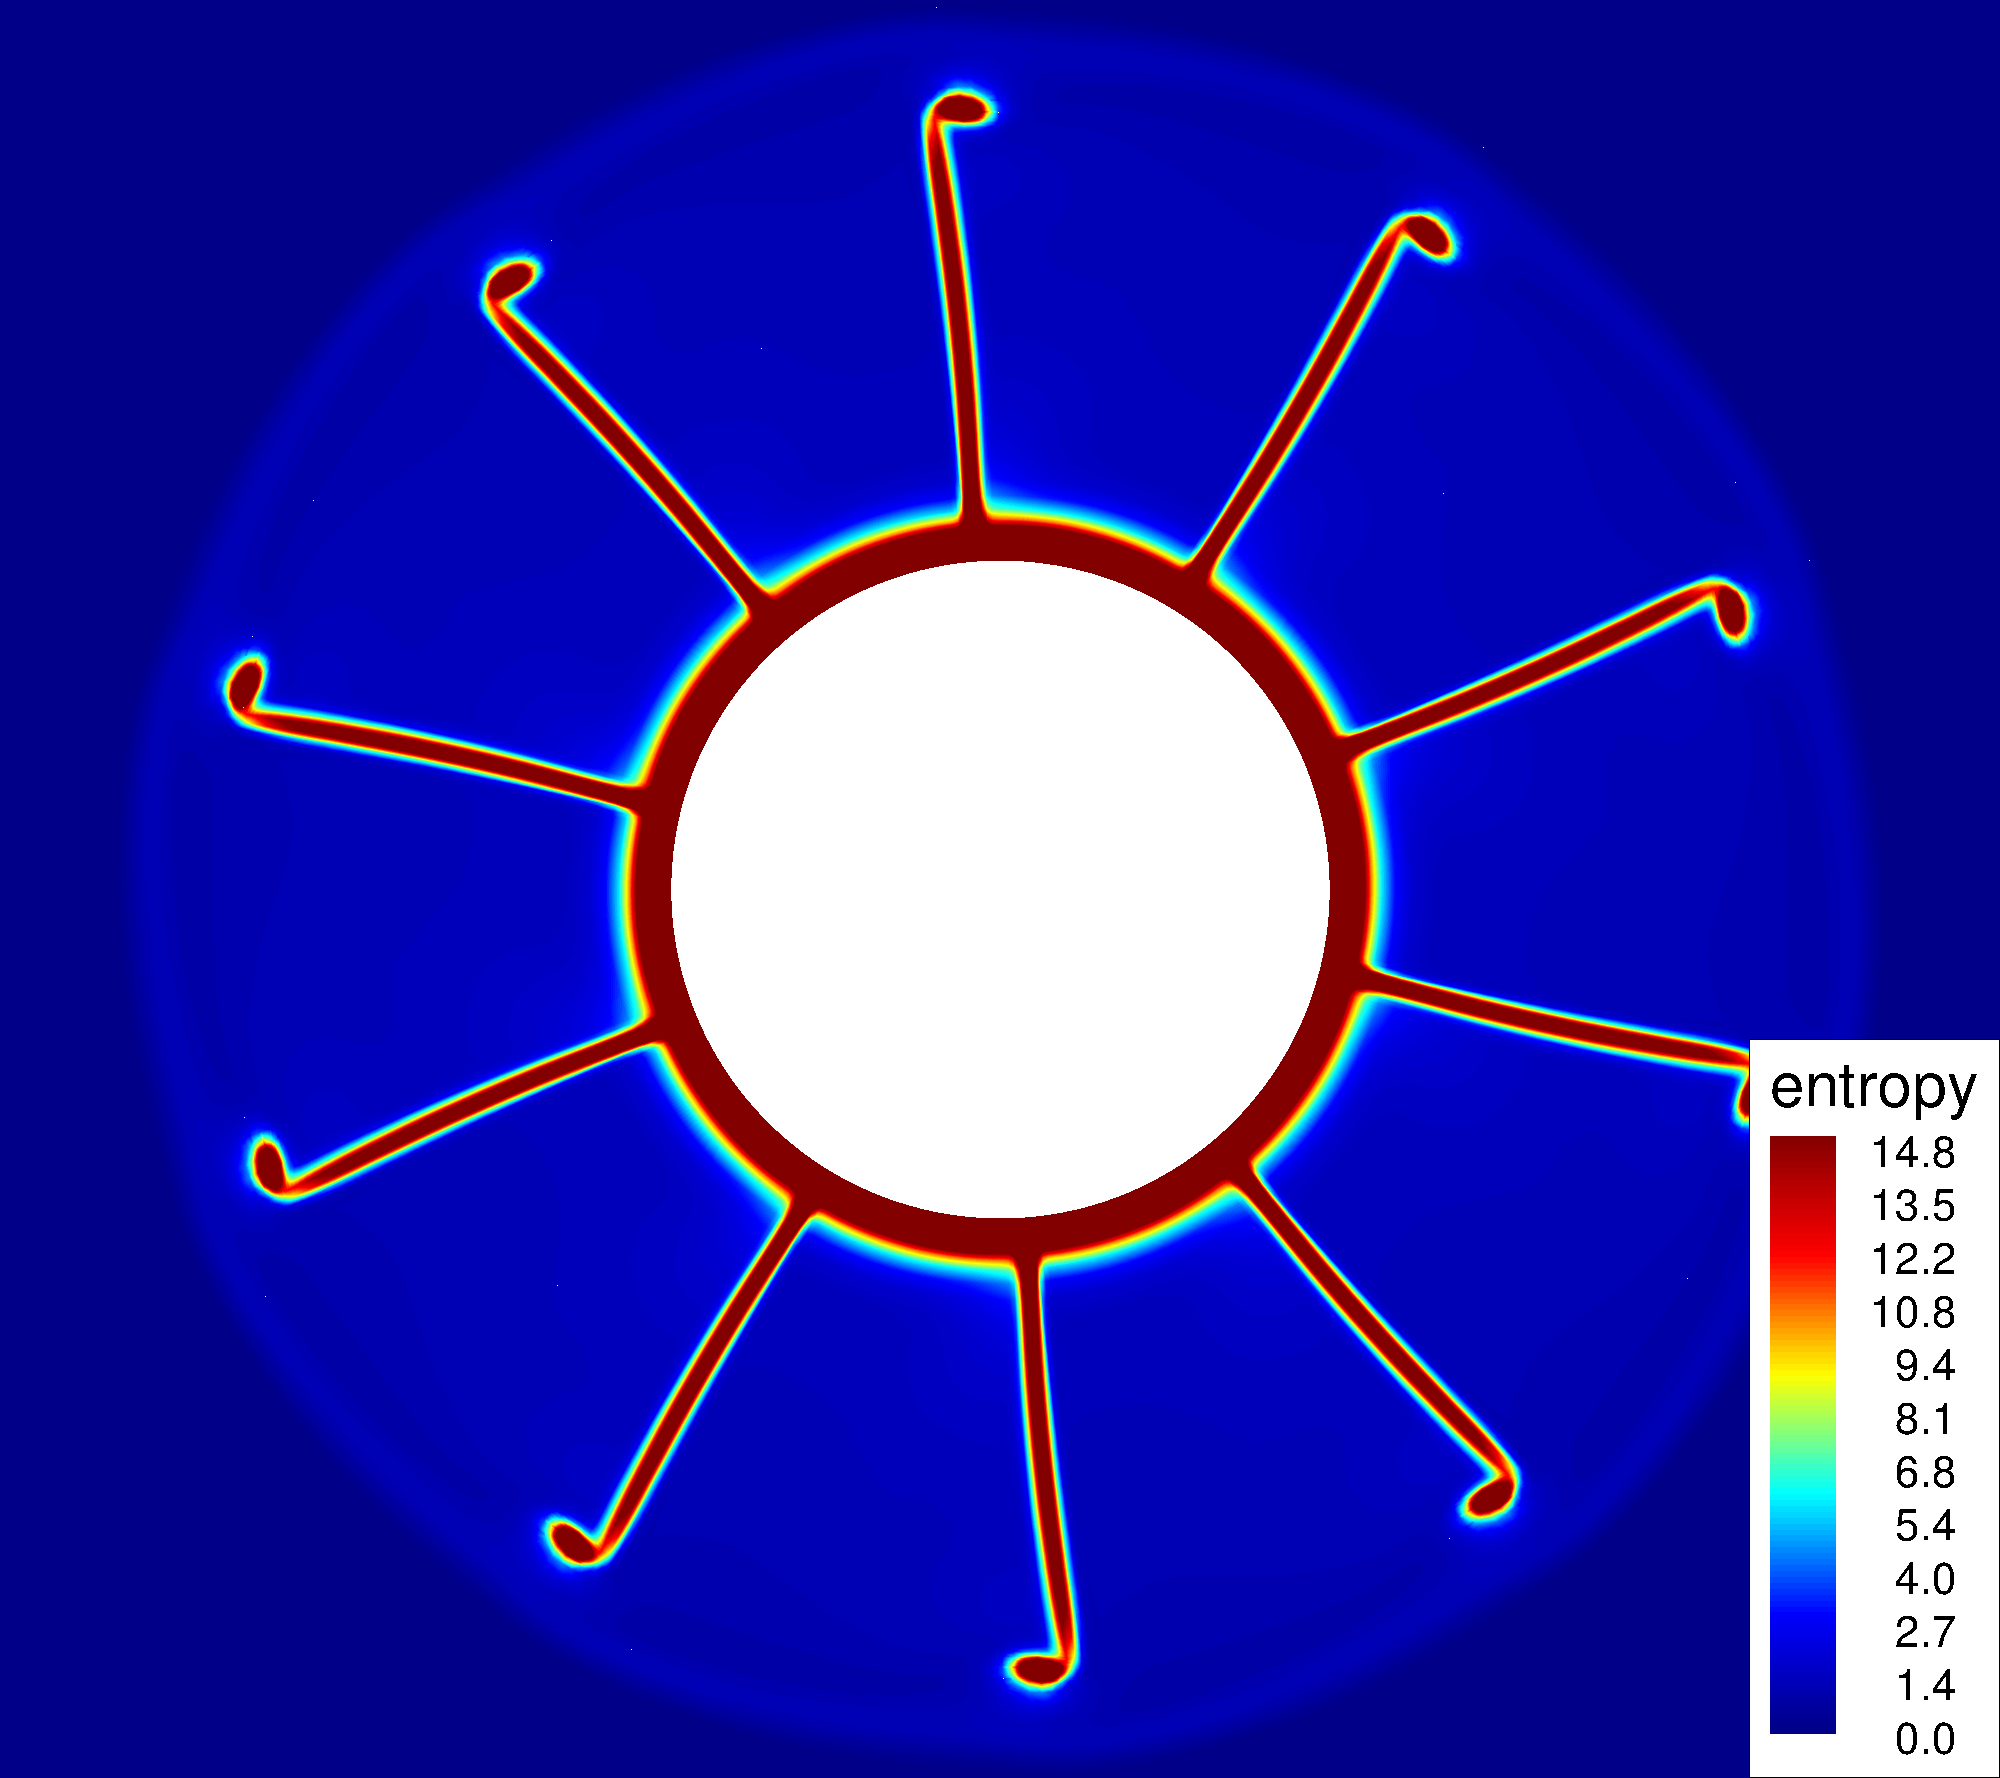
\includegraphics[width=.35\textwidth]{DREAM_HS_RANS_roe2_sa_slice_x_rear_1_entropy.png}
   & 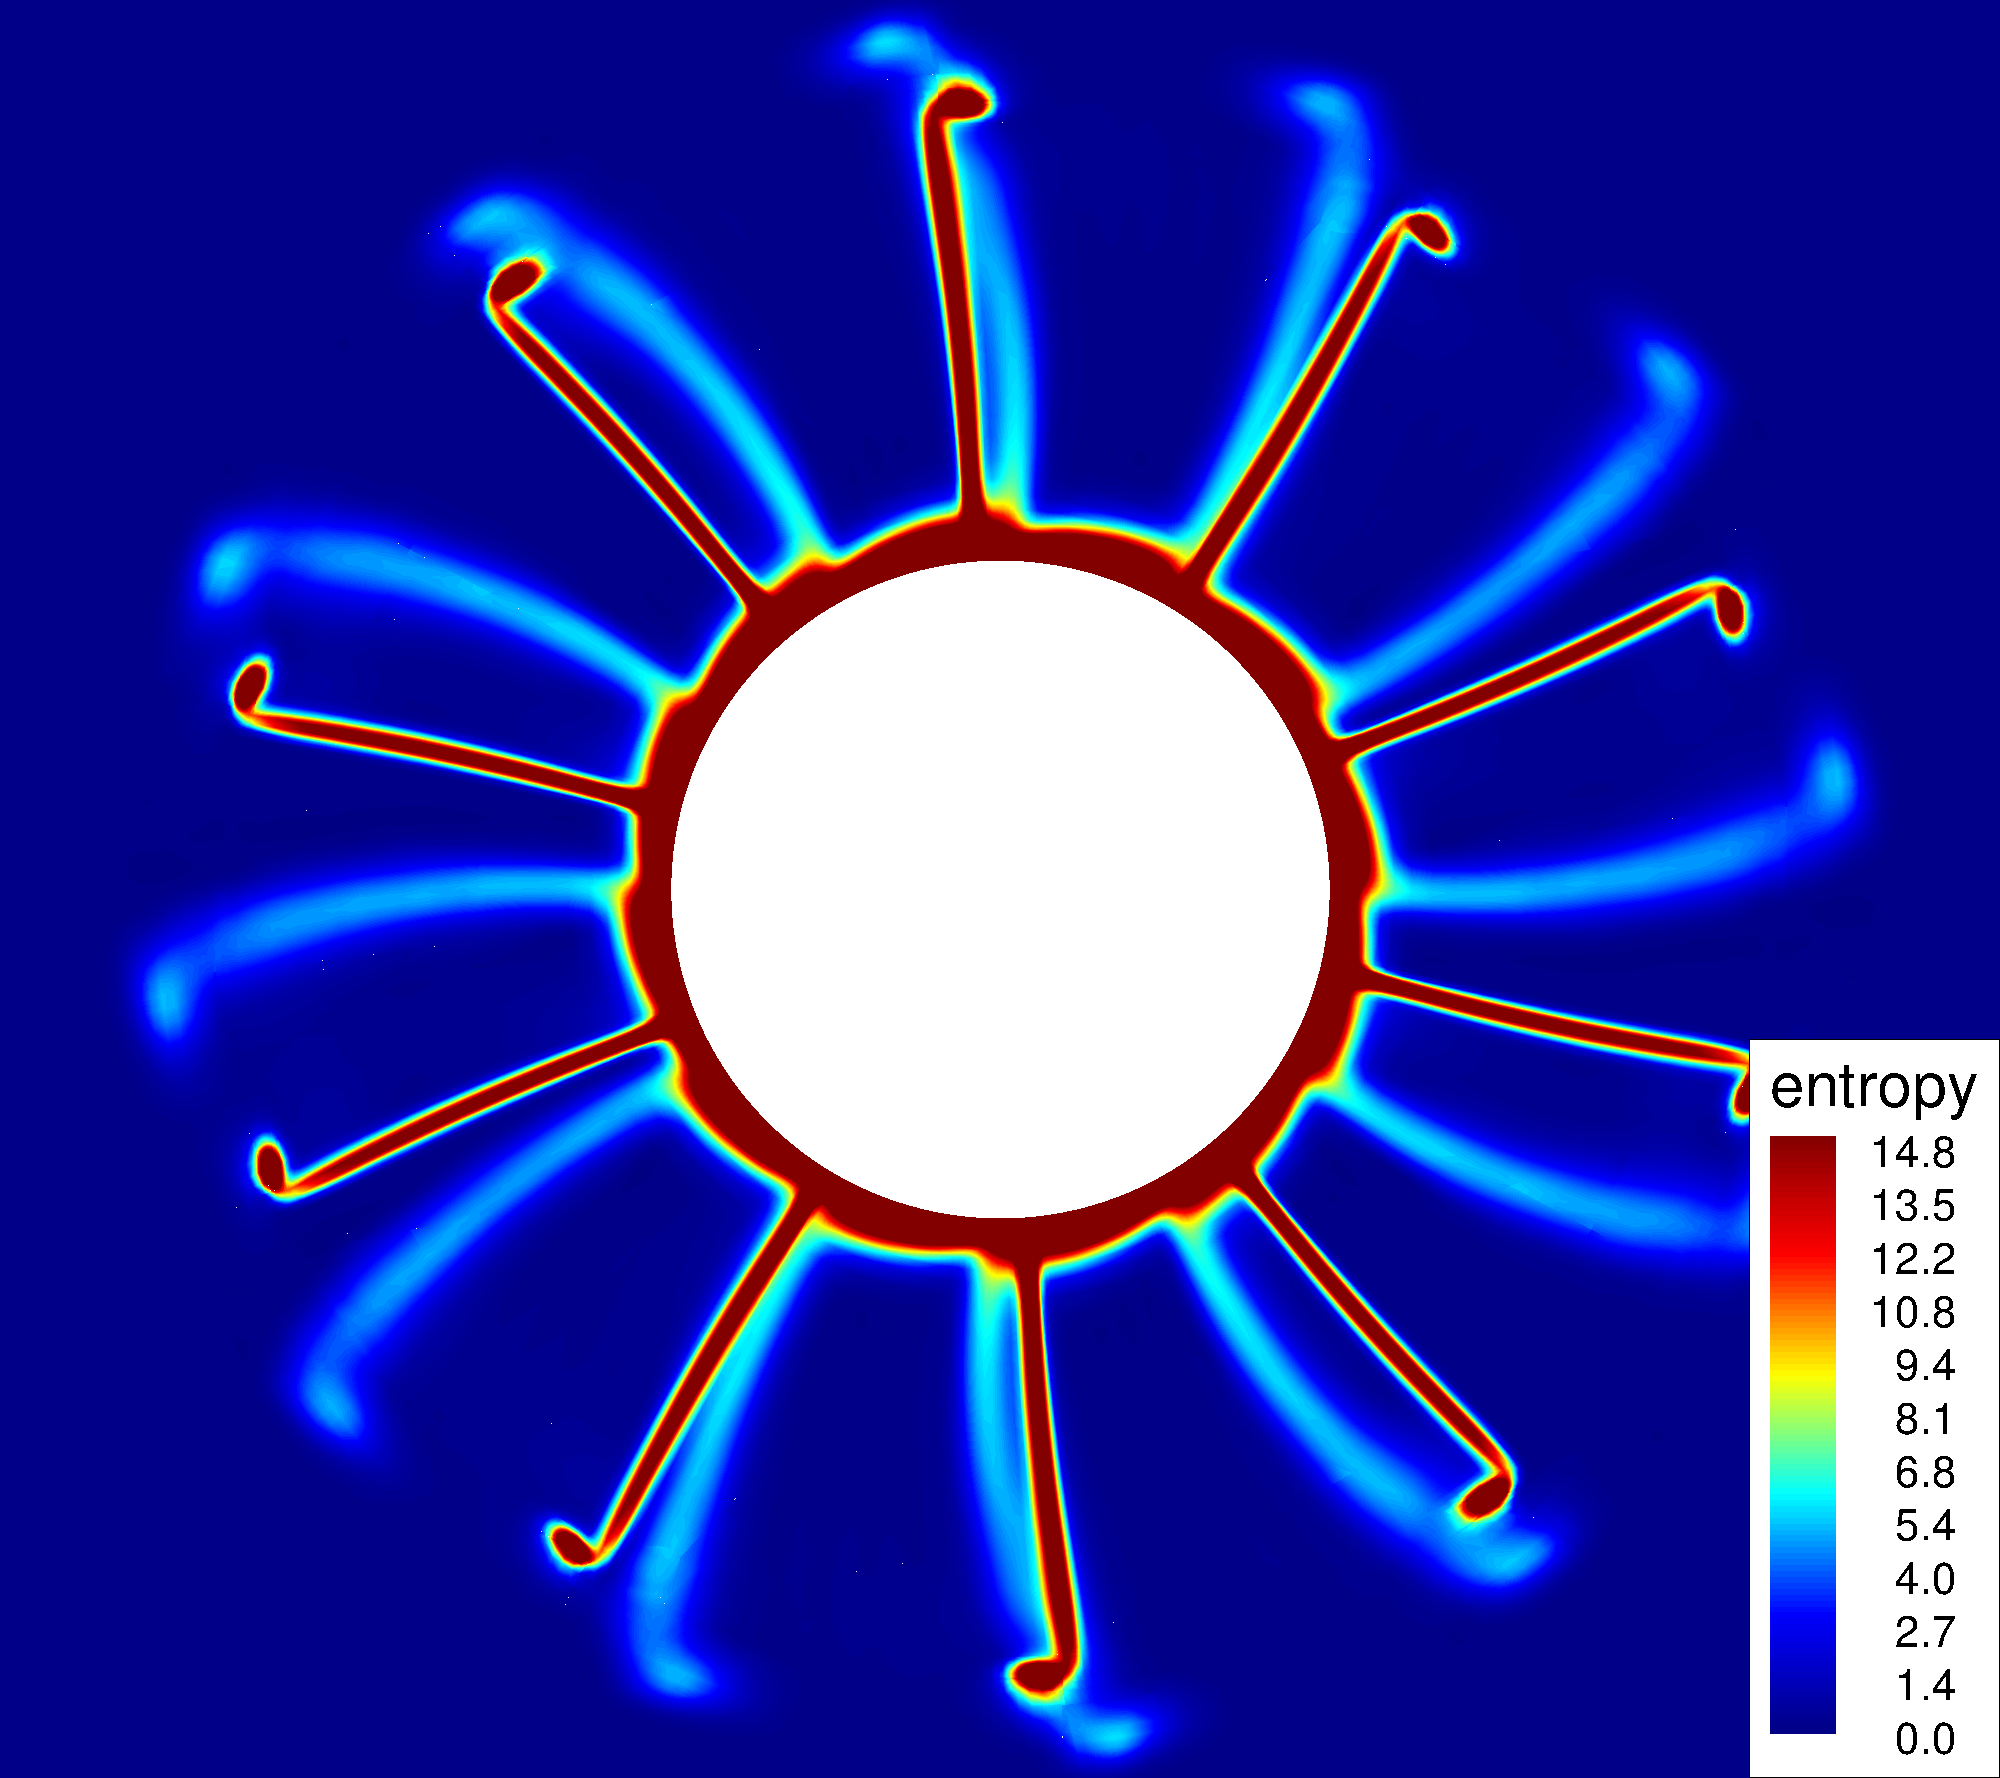
\includegraphics[width=.35\textwidth]{DREAM_HS_TSM_N7_roe2_sa_slice_x_rear_1_entropy.png} \\
   \rotatebox{90}{\qquad\qquad\qquad $P6$} & 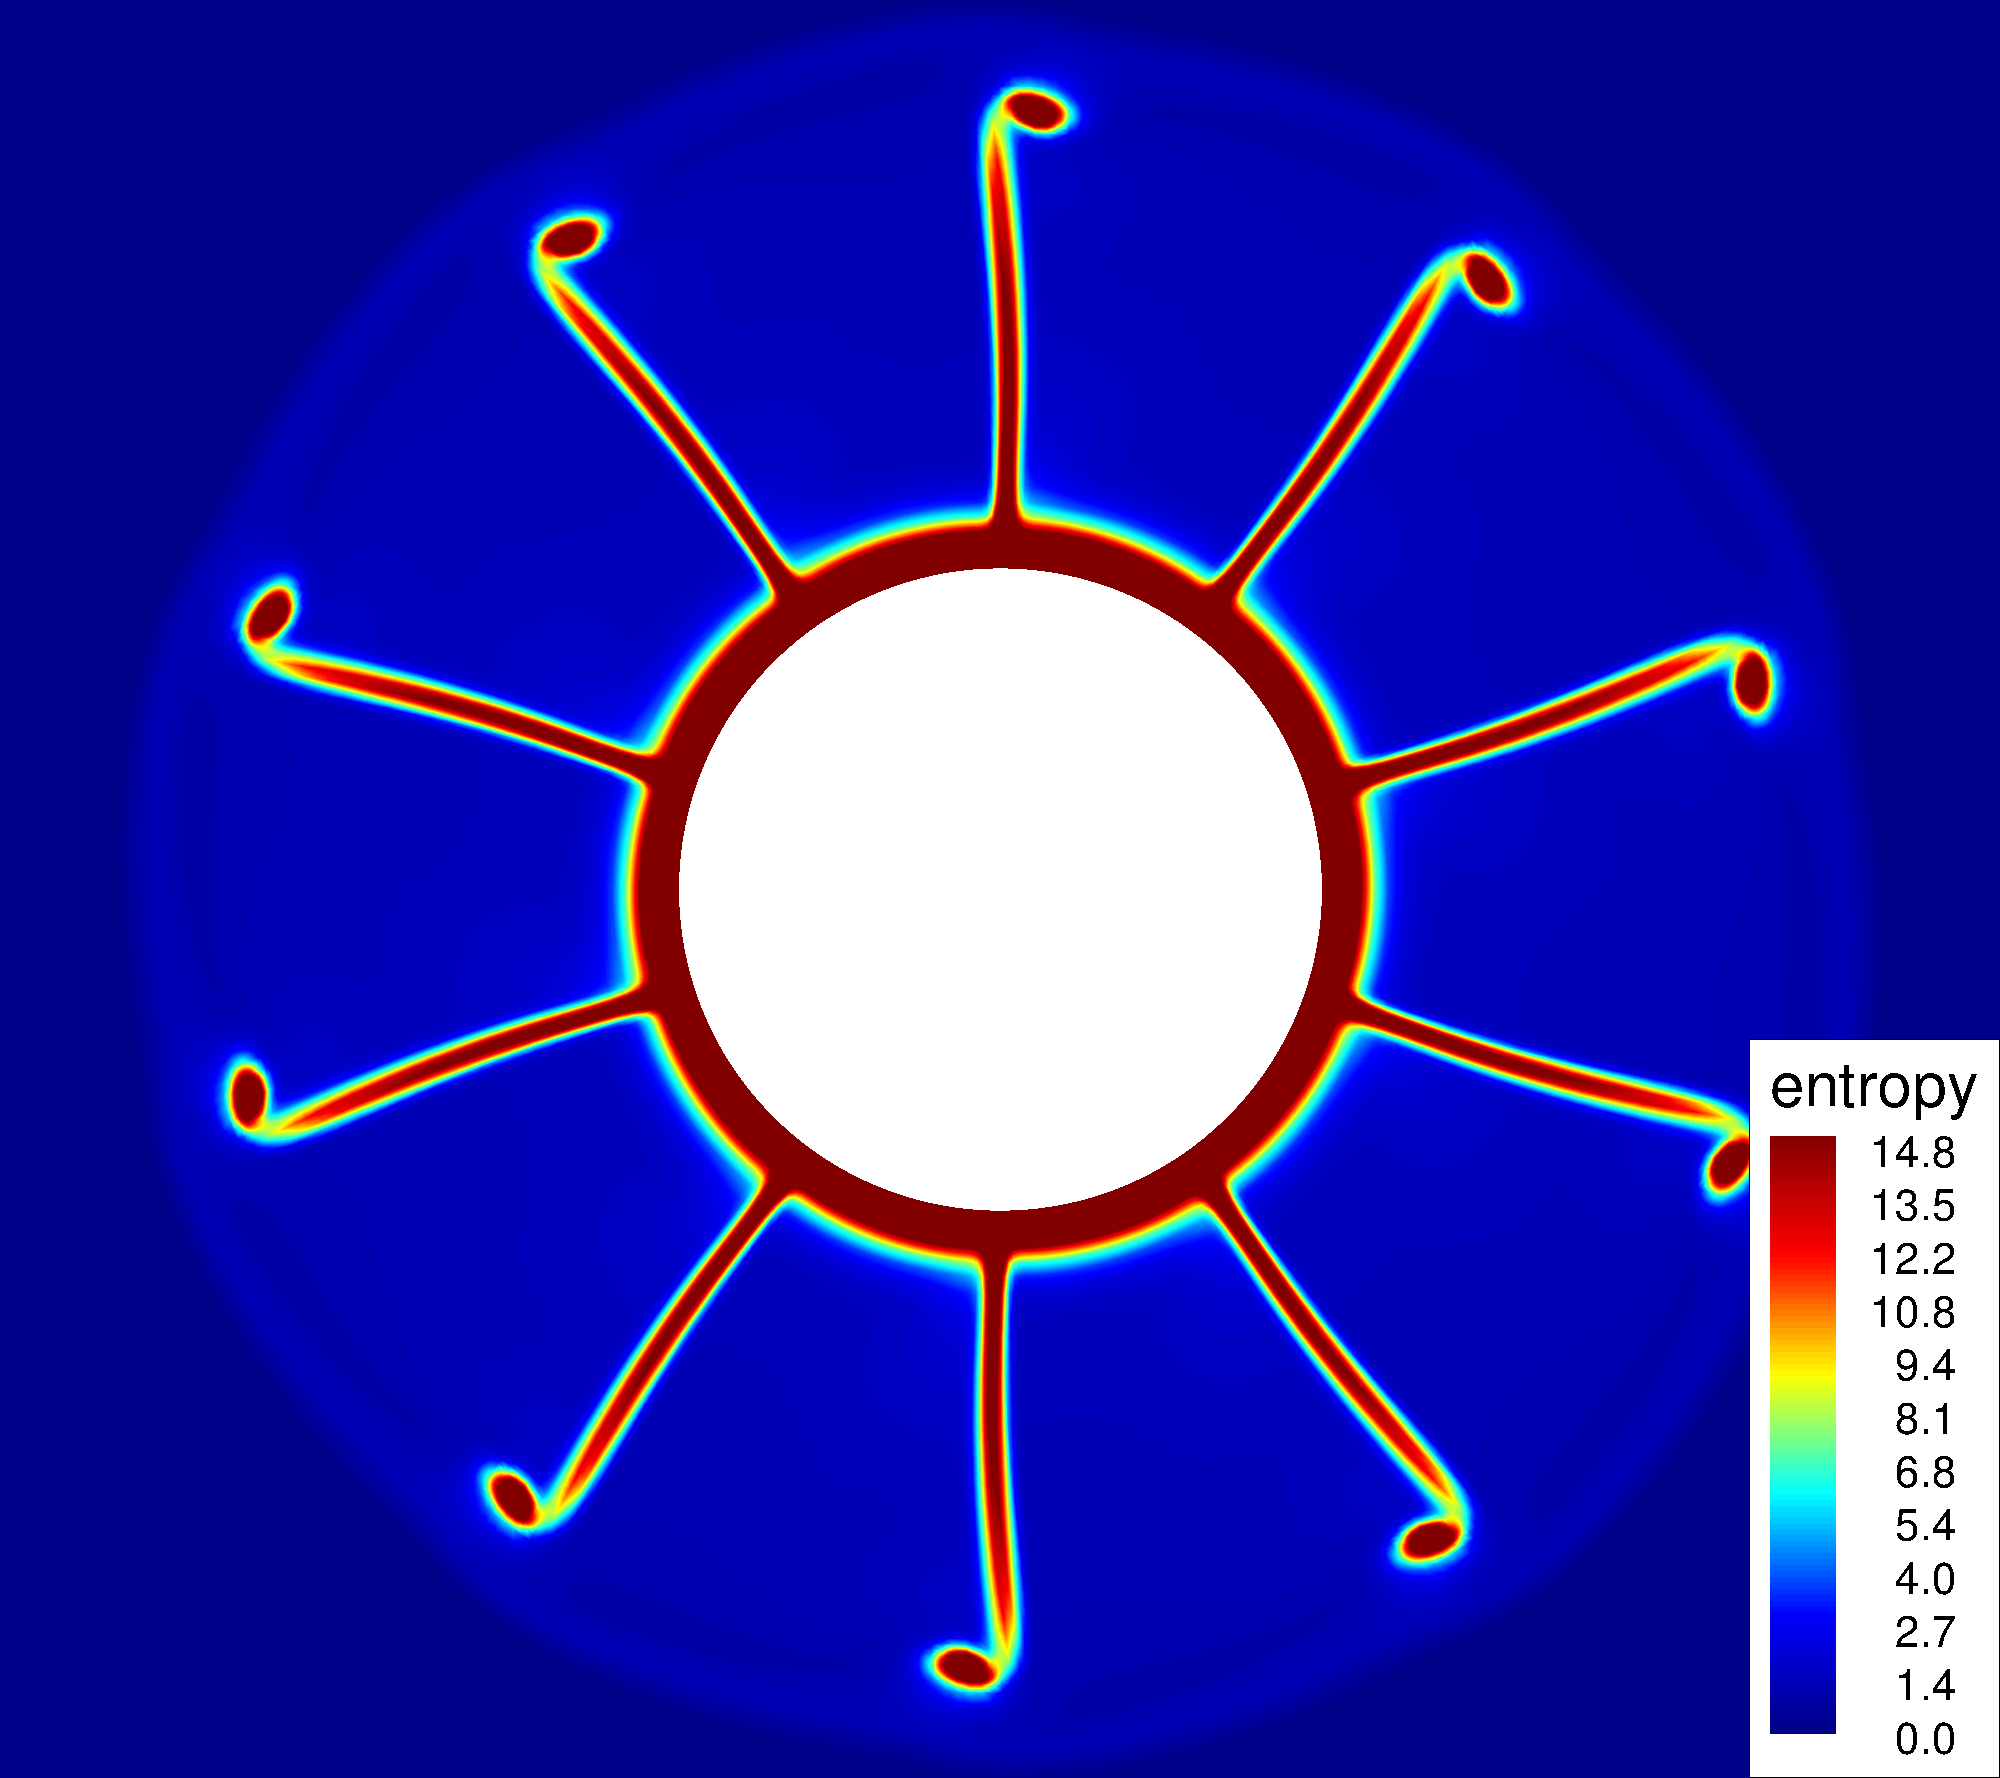
\includegraphics[width=.35\textwidth]{DREAM_HS_RANS_roe2_sa_slice_x_rear_2_entropy.png}
   & 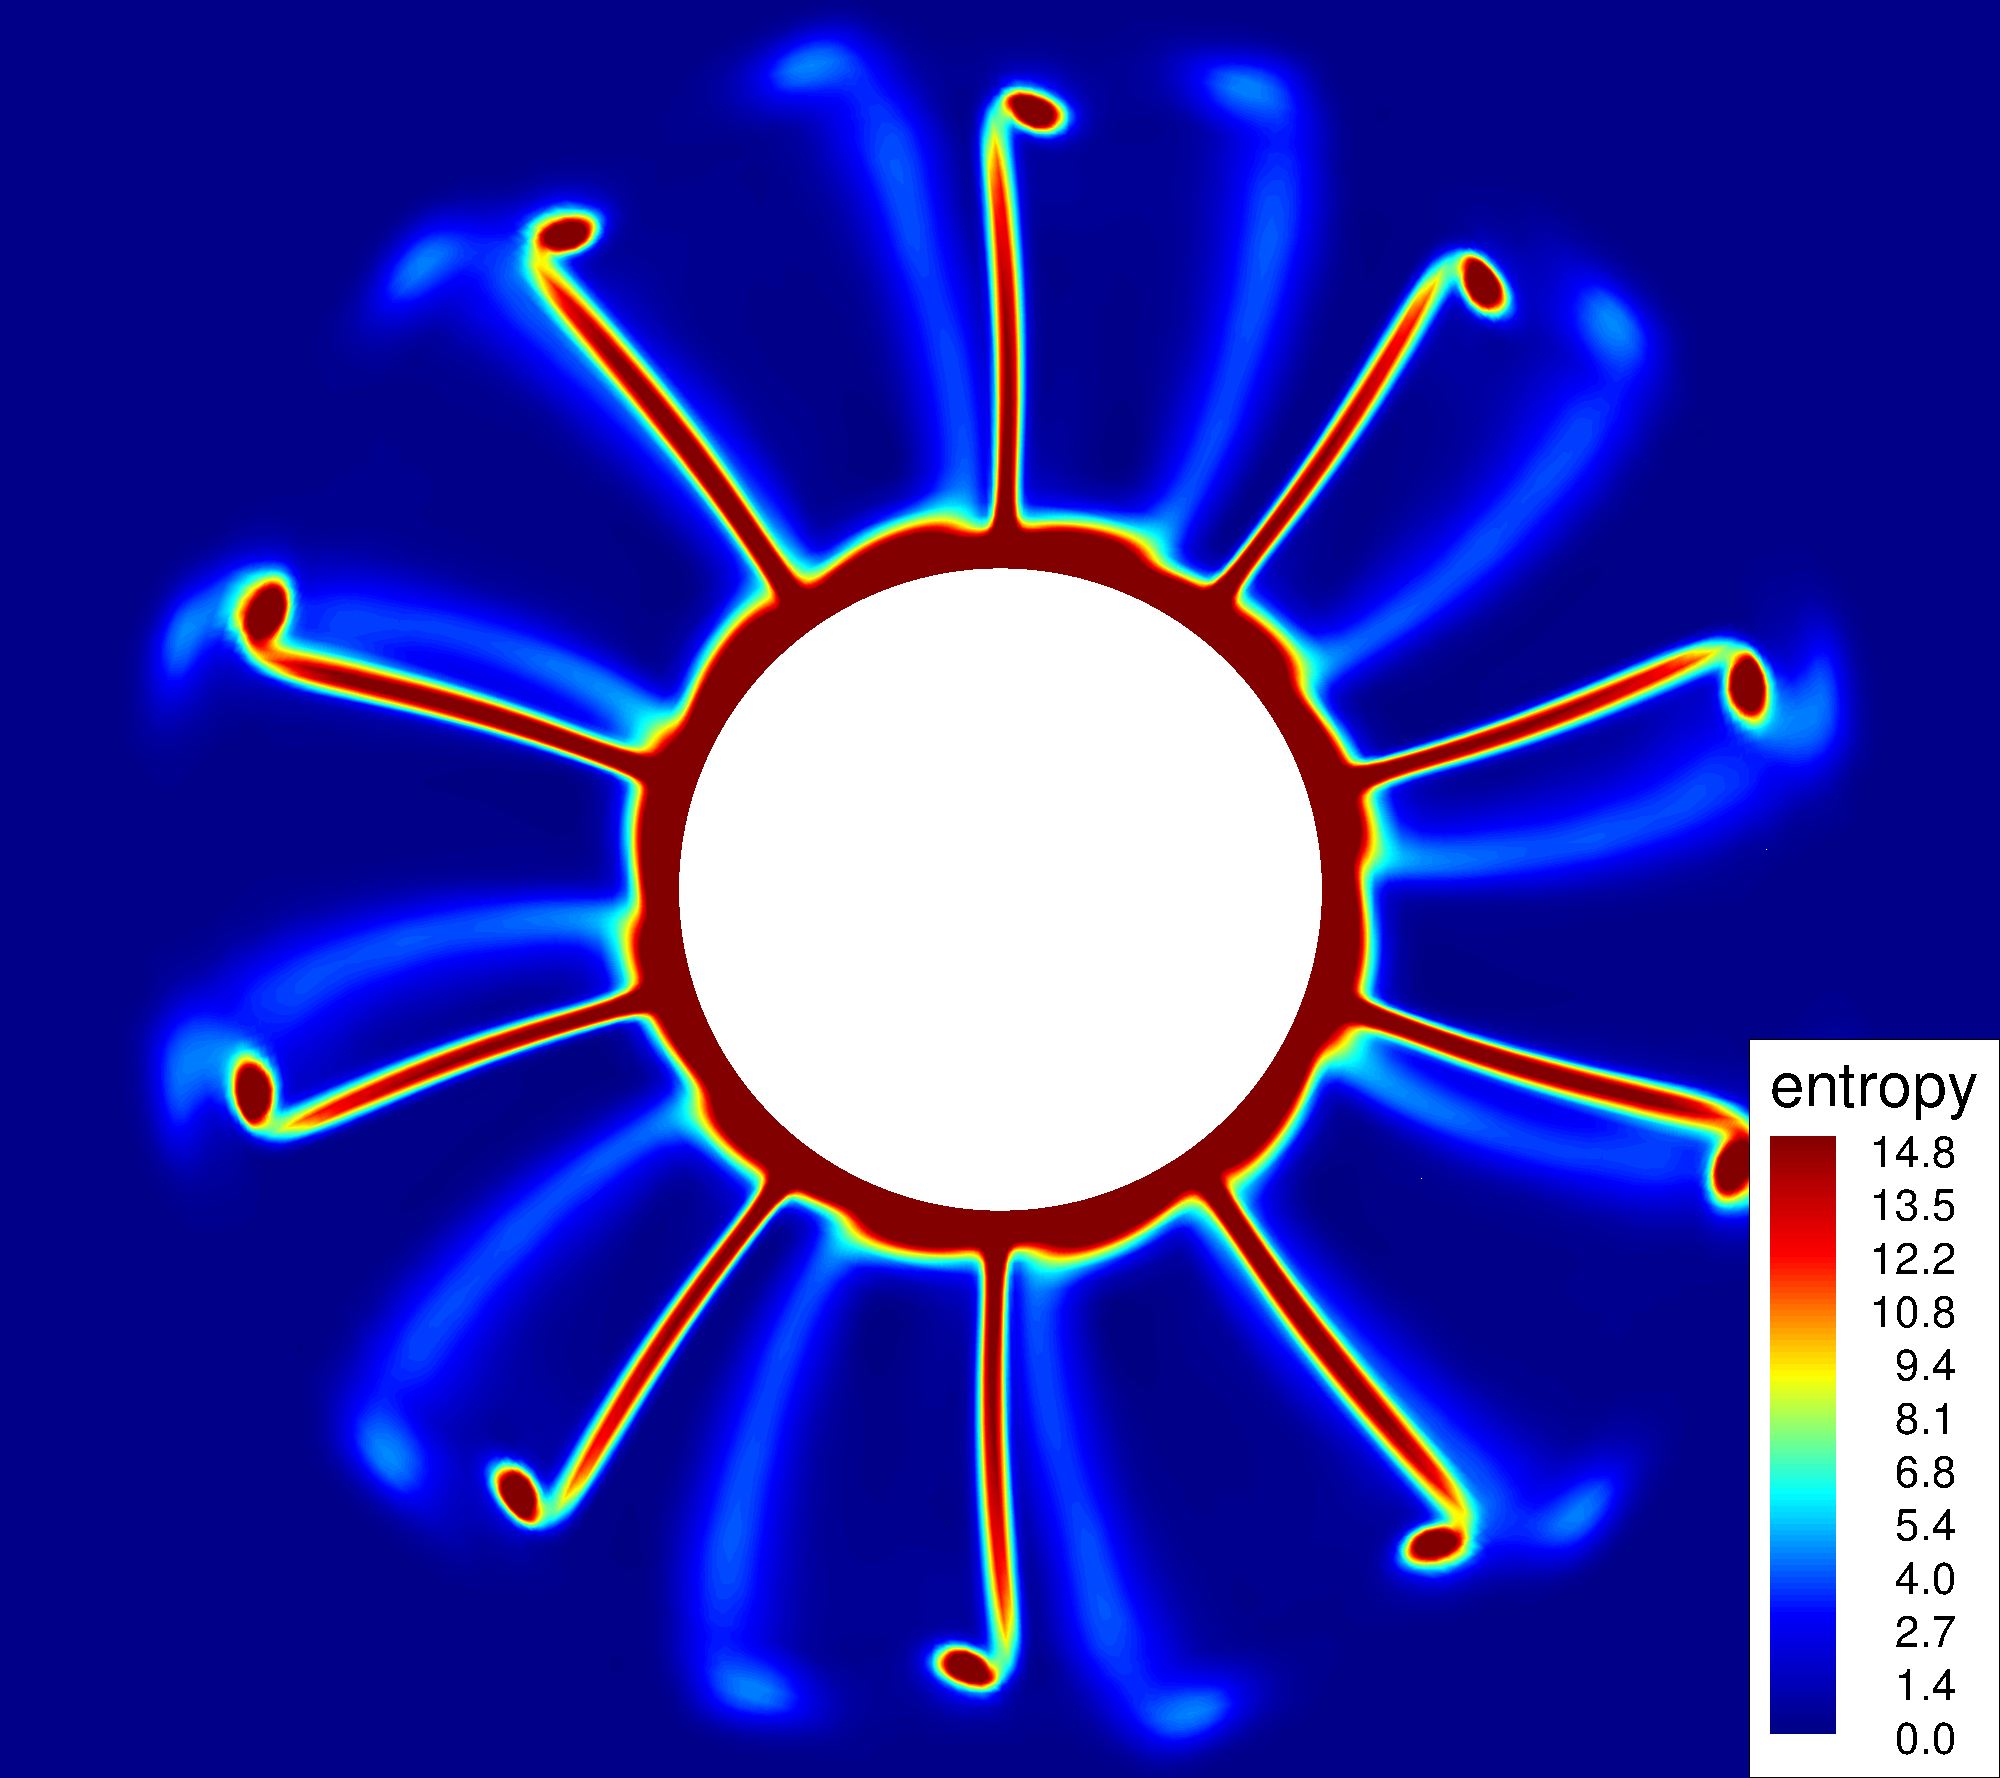
\includegraphics[width=.35\textwidth]{DREAM_HS_TSM_N7_roe2_sa_slice_x_rear_2_entropy.png} \\
 \end{tabular}
 \caption{High-speed isolated configuration: axial cuts of entropy.}
 \label{fig:dream_hs_hb_axial_cut_entropy}
\end{figure}
Clearly, the harmonic balance approach is able to transfer
the tangential distortions between the rows, allowing thus
to capture the interaction of the front tip vortices with
the rear rotor blades. In this high-speed configuration,
the front tip vortex does not hit the rear rotor blades.
The difference with the mixing plane approach is 
tremendous and justifies the use of an unsteady approach
over a steady one. 

One can see that the prediction tool has provided
the number of harmonics needed to ensure the continuity
of the tangential information at the rows interface.
In fact, at the $P4$ plane, no spurious entropy waves
are seen, giving us confidence in the unsteady results.

% \subsection{Two-dimensional results: radial cut of harmonic pressure}
% \label{sub:dream_hs_hb_radial_cuts}

% \begin{figure}[htp]
%   \centering
%   \includegraphics*[width=0.40\textwidth]{DREAM_HS_TSM_N7_roe2_sa_slice_r_70_ps.png}
%   \caption{High-speed isolated configuration: radial cut of the first harmonic of the
%   static pressure normalized by the inflow static pressure.}
%   \label{fig:dream_hs_hb_radial_cuts}
% \end{figure}

% \begin{figure}[htp]
%   \centering
%   \includegraphics*[width=0.40\textwidth]{DREAM_HS_TSM_N7_roe2_sa_slice_r_70_machrel.png}
%   \caption{High-speed isolated configuration: radial cut of the first harmonic of the
%   relative Mach number.}
%   \label{fig:dream_hs_hb_radial_cuts_machrel}
% \end{figure}